\def\Title#1{\textit{#1}}
\def\SCode#1{\Rcode{#1}}
\def\SVariableName#1{\Svar{#1}}
\def\SValue#1{\texttt{#1}}
\def\Email#1{\texttt{#1}}
\def\TabChar{\\t}
\def\NewLineChar{\\n}


\chapter{SPAM: A case study}
%\chapter{Case-Study: Classifying SPAM emails}
\section{Introduction}
 
When we read an electronic-mail message, it is often immediately
obvious to us whether the message is spam or not.  Most of the time we
need only look at the subject line of the message to determine that it
is spam.  But what is not immediately obvious is how to design an
automatic procedure to save us the hassle, time, and irritation of
having to delete ``by hand'' unwanted messages.  In this chapter, we
examine two statistical approaches to classifying electronic-mail
messages as spam or not.

One approach finds the chance a message is spam by looking at which
words are found in the message and which words are absent from it.
This probability-based approach begins by studying the words found in
a large collection of electronic-mail messages which have already been
classified as spam or ham (i.e. not spam).  Then when a new message
comes to us, we use the information gleaned from our ``training'' set
to compute the probability that the message is spam based on the words
appearing in the new message.  We use the naive Bayes method to
compute these probabilities.

The other approach finds the messages in the training set that are
closest to the new message to be classified, and if the majority of
these messages are spam then that message will be classified as spam.
To find close messages, we compute the distance between messages using
particular characteristics, such as the percent of characters in the
message that are capital letters, whether or not the subject line of
the message contains ``Re:'', and the number of attachments.  Then we
find the $k^{th}$ nearest training messages to our new one and use
them in the classification, i.e. if our new message is close to more
spam than ham messages then the new message is classified as spam.
This technique is called $k^{th}$ nearest neighbor classification.

For both of these approaches, we need to ``tune'' the method.
That is, for the naive Bayes method, we must determine a threshold 
for the probability of interest, i.e. for the probability that the message
is spam.
Then a new message is classifed
as spam when the computed chance that it is spam falls above that level, 
otherwise we classify the message as ham.  
To tune the nearest-neighbor method, we must choose $k$, the number of
messages to include in the neighborhood. 
We use the technique of cross-validation to tune these methods.
In addition, we examine the behavior of these classifiers on
a new set of data that has been held in reserve, i.e. not used in the 
training nor in the tuning.

For this case study, we have mail messages from the Spam Assassin website 
\\
\URL{http://spamassassin.apache.org/}.
Altogether, there are five sets of messages: three contain regular
mail (ham) and two contain spam.  Each message is in its own file, and
there are about 9,000 messages in all.  The Spam Assassin Web page,
\URL{http://spamassassin.org/publiccorpus/},
gives a description of the naming convention for the files.

For our first task, we convert the raw text data into an R structure for 
future analysis. 
To do this we consider the following questions:

\begin{itemize}
  \item How should the data be organized?
  \item How do we test our code?
  \item How do we handle special cases?
\end{itemize}

Once the data are in an R structure we begin the application of 
one of the methods. 
For the nearest-neighbor data, we must further process the data
to form quantitative and categorical variables. 
In this process we face several questions,

\begin{itemize}
   \item How do we define a variable?
   \item What is considered a missing value?
   \item How do we check that the variable created is correct?
   \item How do we define a distance between messages based on these variables?
\end{itemize}

On the other hand, for the naive Bayes method, we must further
clean and process our data into a dictionary of sorts. This 
poses its own challenges, 

\begin{itemize}
    \item How do we build a dictionary?
    \item How can we represent the words found in a message in a 
    quantitative way?
    \item How do we check the conversion of text into this quantity?
\end{itemize}

In addition, we address issues common to both approaches, such as 

\begin{itemize}
  \item How do we address efficiency with regard to memory, 
  processing time, and space?
  \item How can we determine whether a method works well or not, and 
  how can we figure out why it works or does not work?
  \item What trade-offs do we face in writing our own high-level code, 
   using other high-level functions and packages, and writing C code?
\end{itemize}

We will address these questions as we work through the main tasks.
We then move on to what has traditionally been considered statistical
work: applying the method, tuning the parameters, and analyzing the
performance of the method on a new set of data.
But, before proceeding, we review how electronic mail works.

\section{The Anatomy of an E-mail message}

Electronic mail, usually called e-mail, consists of simple text
messages -- a piece of text sent to a recipient via the internet.  An
e-mail message consists of two parts, the header and the body.  The
body of the e-mail message is separated from the header by a single
blank line.  When an attachment is added to an e-mail message, the
attachment is included in the body of the message.  Even with
attachments, e-mail messages are still only text messages.

\subsection{The E-mail Header}

The header contains information about the message such as
the sender's address, the recipient's address, and the date of 
transmission.
This information is relayed in a special format 
that consists of  KEY:VALUE pairs.
Below is a sample header from a message found on the
SpamAssassin website.

\begin{verbatim}
Return-Path: whisper@oz.net
Delivery-Date: Fri Sep  6 20:53:36 2002
From: whisper@oz.net (David LeBlanc)
Date: Fri, 6 Sep 2002 12:53:36 -0700
Subject: [Spambayes] Deployment
In-Reply-To: <LNBBLJKPBEHFEDALKOLCIEJABCAB.tim.one@comcast.net>
Message-ID: <GCEDKONBLEFPPADDJCOECEHJENAA.whisper@oz.net>
\end{verbatim}
                                                                               
Notice the keys are Return-Path, Delivery-Date, From, Date,
Subject, In-Reply-to, and Message-ID. 
The value follows the keyword.
For example, in the above header, the value of the From key 
is \\
\texttt{whisper{at}oz.net (David LeBlanc)}.

Some of these keys are mandatory such as \Email{Date, From}, and \Email{To} 
(or \Email{In-Reply-To}, or \Email{Bcc}).
Other keys are optional but widely used, such as \Email{Subject, Cc, 
Received}, and \Email{Message-ID}.
Many keys are ignored by the mail system, but the entire header 
is relayed on to the recipient's server whether or not it is 
recognized. 
For example, keys starting with ``\Email{X}-'' are for personal application 
or institution use and are ignored by other applications.
The \Email{Received} header lines are important because they allow
the message to be tracked. As a message makes its way to the
intended recipient, servers add additional \Email{Received} lines
to the header. 


Below are some typical header keys:

\begin{itemize}
\item \Email{Message-Id}: a unique identifier for the message, assigned by the 
originating server; 
\item \Email{Return-Path}: specifies the sender's address and  
        bounced mail gets sent to this address;
\item \Email{Date}: added by the e-mail client;
\item \Email{Cc}: lists the recipients of a ``carbon copied'' message;
\item \Email{Reply-To}: the address set by the sender to which the 
recipient can reply; 
\item \Email{MIME-Version}: used for encoding binary content as attachments.
\end{itemize}

A value may be continued on a second line of the header, in which
case the line will be indented and begin with a tab character or
blank spaces.

\subsection{E-mail Attachments}

An Internet standard called MIME, 
Multipurpose Internet Mail Extensions, 
specifies how messages may be formatted and how to separate 
the attachments from the message. 
Information about the MIME encoding is provided through header fields, 
which are specified in an RFC. 

The Content-Type key is used to describe the content of a component
or of the entire body. 
The value provides the top-level type and subtype using the 
syntax:  
\begin{verbatim}
top-level/subtype; parameter.
\end{verbatim}
Parameters may be required or optional.
Below is an example of a content-type where the 
top-level is \Email{multipart}, which indicates there will be several 
documents in the body of the message, the \Email{mixed} subtype tells
us that the documents may be of different types, and the \Email{boundary}
parameter provides a special character string for delimiting the
start and end of the message parts.
\begin{verbatim}
Content-Type: multipart/mixed;
      boundary="----=_NextPart_000_00DE_01511A02.DB1A02A0"
\end{verbatim}
The Content-Type field in this example tells the receiving 
e-mail program that this message has more than one component, and each 
component will be separated by the string of characters 
\begin{verbatim}----=_NextPart_000_00DE_01511A02.DB1A02A0\end{verbatim}
The boundary string marks the beginning of each component.
It is prefaced with two additional hyphens in all instances.
The boundary string is also used to denote the end of the message, 
where it is both prefaced by two hyphens and followed immediately by two 
hyphens. 
The receiving email program knows when the last component of the message
has been read when it reads the boundary string with two additional
hyphens on either end of the string,
\begin{verbatim}------=_NextPart_000_00DE_01511A02.DB1A02A0--\end{verbatim}
Each component of a message must be prefaced by the boundary string
and a blank line. 
It may also contain MIME information.
If the blank line is missing, the recipient's e-mail client may have 
difficulty telling where the header information stops and the text of the 
message begins.

There are seven top-level types of attachments: text, image, audio, video, application,
multipart, and message.  Other examples of Content-Type values follow:

\begin{verbatim}
Content-type: text/html; charset=euc-kr;
Content-Type: application/zip; name="testFile.zip"
\end{verbatim}
The first example indicates that the message is in HTML format using a
Korean character set.  The second indicates that the component
is a zip file, and the sender named it \File{testFile.zip}.
Binary files (such as a compressed archive) can be
sent as attachments. 
In such cases, the sender's software must first encode the binary
file so that it can be sent over the Internet. 
One common encoding scheme is known as base64. 

We conclude by providing two sample e-mail messages.
The first is a plain text e-mail with no
attachments.  It consists of an instructor's response
to an e-mail inquiry sent by a student. 
The second e-mail message consists of a text message and two attachments 
sent by a student to the instructor. This e-mail message has then been 
forwarded by the instructor to the teaching assistant.
The three periods at the end of each attachment indicates
that only part of the attachment has been displayed.
The first attachment is a pdf file and the second is an HTML file.
The forwarded message is a plain text file.

\begin{figure}

%\framebox{
{\small{
\begin{verbatim}
 
From nolan@stat.Berkeley.EDU Mon Feb  2 22:16:19 2004 -0800
Date: Mon, 2 Feb 2004 22:16:19 -0800 (PST)
From: nolan@stat.Berkeley.EDU
X-X-Sender: nolan@kestrel.Berkeley.EDU
To: Txxxx Uxxx <txxxx@uclink.berkeley.edu>
Subject: Re: prof: did you receive my hw?
In-Reply-To: <web-569552@calmail-st.berkeley.edu>
Message-ID: <Pine.SOL.4.50.0402022216120.2296-100000@kestrel.Berkeley.EDU>
References: <web-569552@calmail-st.berkeley.edu>
MIME-Version: 1.0
Content-Type: TEXT/PLAIN; charset=US-ASCII
Status: O
X-Status:
X-Keywords:
X-UID: 9079
  
Yes it was received.
 
-------------------------------------
 
On Mon, 2 Feb 2004, txxxx wrote:
 
> hey prof .nolan,
>
> i sent out my hw on sunday night. i just wonder did you receive it.
> because i am kinda scared thatyou didnt' receive it.
> like i just wonder how do i know if you got it or not, since the cal
> mail system is kinda weird sometimes.  thanks
>
> txxxx
>
\end{verbatim}    
} }
% }
\caption{Sample email message with no attachments. The header includes fourteen
key:value pairs.  Note the \Email{Date} key includes a time-zone offset,
the \Email{Message-ID} key gives the unique ID to track the
mail from the \URL{stat.berkeley.edy} mail server,
the \Email{Content-Type} key indicates it is a plain text message
with no sttachments, and thre are four \Email{X-} keys.}\label{fig:simpleEmail}
\end{figure}


\begin{figure}
{\footnotesize{
\begin{verbatim}
From nolan@stat.Berkeley.EDU Mon Feb  2 22:18:56 2004 -0800
Date: Mon, 2 Feb 2004 22:18:55 -0800 (PST)
From: nolan@stat.Berkeley.EDU
X-X-Sender: nolan@kestrel.Berkeley.EDU
To: Gang Liang <liang@stat.Berkeley.EDU>
Subject: Assignment 1 sorry (fwd)
Message-ID: <Pine.SOL.4.50.0402022218470.2296-201000@kestrel.Berkeley.EDU>
MIME-Version: 1.0
Content-Type: MULTIPART/Mixed; BOUNDARY="_===669732====calmail-me.berkeley.edu===_"
Content-ID: <Pine.SOL.4.50.0402022218471.2296@kestrel.Berkeley.EDU>
Status: RO
X-Status:
X-Keywords:
X-UID: 9080
 
--_===669732====calmail-me.berkeley.edu===_
Content-Type: TEXT/PLAIN; CHARSET=US-ASCII; FORMAT=flowed
 
Content-ID: <Pine.SOL.4.50.0402022218472.2296@kestrel.Berkeley.EDU>
\end{verbatim}
}}
\caption{This sample email (split over two figures) has two
  attachments, a PDF file and an HTML file.  The \Email{Content-Type}
  key indicates that the attachments are separated by
  \Email{\_===669732====calmail-me.berkeley.edu===\_} with a
  \Email{--} prefix.  The first part of the email body is the a
  forwarded message.  Note that it has its own header indicating the
  content type is plain text.  Next is a PDF attachment which the
  owner has named \FileName{PLOTS.pdf}, and the third part is an HTML
  attachment.  Both attachments are encoded in base64.  }
\end{figure}

\begin{figure}
{\footnotesize{
\begin{verbatim}

---------- Forwarded message ----------
Date: Mon, 02 Feb 2004 21:50:47 -0800
From: Yyyy Zzz <Zzz@uclink.berkeley.edu>
To: nolan@stat.Berkeley.EDU
Subject: Assignment 1 sorry
 
I am sorry to send this email again, but my outbox told me that 
the last email only send 1 attached file. 
I am send ing this again to make sure you recieve the all 
the necessary files.
Thank You and sorry for the inconvenience.
  
--_===669732====calmail-me.berkeley.edu===_
Content-Type: APPLICATION/PDF; CHARSET=US-ASCII
Content-Transfer-Encoding: BASE64
Content-ID: <Pine.SOL.4.50.0402022218473.2296@kestrel.Berkeley.EDU>
Content-Description:
Content-Disposition: ATTACHMENT; FILENAME="PLOTS.pdf"
 
JVBERi0xLjEKJYHigeOBz4HTDQoxIDAgb2JqCjw8Ci9DcmVhdGlvbkRhdGUgKEQ6MjAwNDAy
MDIxMTIwMTEpCi9Nb2REYXRlIChEOjIwMDQwMjAyMTEyMDExKQovVGl0bGUgKFIgR3JhcGhp
Y3MgT3V0cHV0KQovUHJvZHVjZXIgKFIgMS44LjEpCi9DcmVhdG9yIChSKQo+PgplbmRvYmoK
...
 
--_===669732====calmail-me.berkeley.edu===_
Content-Type: TEXT/HTML; CHARSET=US-ASCII
Content-Transfer-Encoding: BASE64
Content-ID: <Pine.SOL.4.50.0402022218474.2296@kestrel.Berkeley.EDU>
Content-Description:
Content-Disposition: ATTACHMENT; FILENAME="Stat133HW1.htm"
  
PGh0bWwgeG1sbnM6bz0idXJuOnNjaGVtYXMtbWljcm9zb2Z0LWNvbTpvZmZpY2U6b2ZmaWNl^M
PGh0bWwgeG1sbnM6bz0idXJuOnNjaGVtYXMtbWljcm9zb2Z0LWNvbTpvZmZpY2U6b2ZmaWNl^M
Ig0KeG1sbnM6dz0idXJuOnNjaGVtYXMtbWljcm9zb2Z0LWNvbTpvZmZpY2U6d29yZCINCnht^M
...

--_===669732====calmail-me.berkeley.edu===_--
    
\end{verbatim}
}}
\caption{This sample email (split over two figures) has two
  attachments, a PDF file and an HTML file.  The \Email{Content-Type}
  key indicates that the attachments are separated by
  \Email{\_===669732====calmail-me.berkeley.edu===\_} with a
  \Email{--} prefix.  The first part of the email body is the a
  forwarded message.  Note that it has its own header indicating the
  content type is plain text.  Next is a PDF attachment which the
  owner has named \FileName{PLOTS.pdf}, and the third part is an HTML
  attachment.  Both attachments are encoded in base64.  }
\end{figure}

\section{Converting raw text data into an R structure}
Whether it be naive Bayes classification or $k^{th}$-nearest
neighbor, the first task we face is to convert the raw text data into 
an R structure for further processing and analysis.

\subsection{Organizing the Data}
To get started we want to think about what we want to end up with
in terms of a data structure. 
If we just start writing code, there is a
danger that we will get confused and the code will become inter-twined
with doing several different things.  
So what type of data structure do we want?
Of course it depends on what we want to do with the data in the future, 
but a reasonable structure to create might be a
collection of R objects with one object for each mail message.  
Then, each message-object might have the following four elements: 

\begin{itemize}
\item \textit{The contents of the header}  The header elements tell us
about the sender, recipient(s), date sent, routing information 
of the message, mail program used to compose the message, etc.
Since we want to deal with the header in terms of its key-value pairs, 
it seems easiest to represent the contents of the header as 
a named character vector where the name of an element corresponds 
to the key and the character string corresponds to the value for that key.

\item \textit{The message text or body}
The message text does not require any special processing.
Simply maintaining is as a collection of text lines at this
point seems most expedient. 

\item \textit{The attachments in the message}
We want to handle the attachmens in the message
separately from the text in the body of the message. 
Also, as each attachment has its own mini-header, we will want the header 
and body of the attachment handled in a manner parallel to the message header
and body.  

\item \textit{An indicator for spam} 
We want the information as to whether the message is spam or ham
part of the message-element. A logical value seems an appropriate 
data type.  
In its original form, 
this information must be determined from the name of the directory 
that contains the email message file.

\item \textit{File name} 
While the filenames of the messages are not relevant to processing
their contents, it is often useful when debugging to be able to ask
for the name of the file in which a message was located.  This allows
us to easily identify and view the source and compare it with the
resulting S object that we compute.
So we will also put in the name of the file for each message. 
\end{itemize}

Given these constraints, it makes sense to store the data as a list
with one element for each message and an element name that matches
the filename of the message.  (See Figure \ref{fig:spamStructure}.)
Each element will itself be a list containing a named character vector
for the header, a logical indicating if the message is spam or not,
and another list for the body.
This list will have one element for the body which will be a 
character vector that contains one line for each text line in the body,
and if the message has attachments, an attachment element.
The attachment element will have a structure that is parallel to
the main structure of the email.  That is, the attachment element will
be a list with one element per attachment, each of which is a list of 
two elements, a header character vector and a body character vector.

\begin{figure}

\vspace{3in}

\caption{Data Structure for the email messages found in Figure~\ref{fig:simpleEmail}}\label{fig:spamStructure}
\end{figure}

\subsection{Organizing the tasks to create the data structure}

While the overall task is to process all the messages, 
we should develop our code by reading in just a few messages.  
We develop our code in separate
units, namely functions, to process individual messages and then
gradually work up or out-wards to process all of the messages.  These
top-level steps are merely loops over the directories and the
individual messages within each of the 5 directories that contain the
email messages.  The function
for reading an individual message should be the same for all
directories and messages. So we focus on that first and 
try to handle special cases as we encounter them.

\subsubsection{Identifying Subtasks}
At its simplest, we identify the steps needed to process an individual
email message.

\begin{itemize}
\item 
 \textit{read} the lines of the message from the file;

\item
 \textit{split} the message into the header part and the body part;

\item
 \textit{convert} the header into a vector of named values so 
 we can explore the fields later across all messages.
\end{itemize}
Note that we ignore the handling of the attachments for now.
The complete code, which appears in Section~\ref{sec:SpamCode},
includes the code for processing email attachments.

One of the useful characteristics of languages like R and Matlab is
that they are interactive and allow us to try commands at the prompt,
correct and perfect them and then add them to functions in an editor.
So we open an editor and create a function for reading an individual 
message.  
We will call this function \SVariable{splitMessage} as it
will read in a message and split it up into appropriate pieces.  
To define the function,
we need to use the \Sfunc{function} keyword and specify
the list of formal arguments and the body of the function.  We assign
the resulting function to \SVariable{splitMessage}.

\begin{verbatim}
splitMessage = function() 
{
}
\end{verbatim}

\subsubsection{Identifying Inputs}
The list of formal arguments to the function typically grows as we 
write functions,
and usually we add convenience arguments or options to control how it
reports information or what it actually does.  When we start to write
a function, we determine what are the essential inputs.  In this case,
we need the name of the file that is to be read so our function
\SVariable{splitMessage} takes one argument, \SVariable{fileName},
which holds the name of file to be read.

\begin{verbatim}
splitMessage = function(fileName) 
{
}
\end{verbatim}


\subsubsection{Sample Data}
Before we can get started, we have to find a message file
with which we can experiment.  One thing to do is simply put the
the messages wherever you want them to make things easy to get
started, but in the end, we will want to read them from
an installed R package so that our code will work on different machines
and not be dependent on having the files in a particular directory
name. After all, we do want the code to work on different machines for
different people so that if we return to it, we don't have to spend
time recalling our original configuration.

If we want to find the files in a machine-independent
manner now and not access them directly from our own copy 
of the zip or tar file, then we explore ways to find the files.
A clean way is  to use 
\Sfunc{system.file}
to find the full path name of a file or directory in an installed package.
\begin{verbatim}
> library(RSpamDataMini)
> system.file("messages", DirectoryNames, 
              package = "RSpamDataMini")
[1] "/home/duncan/tmp/RSpamDataMini/messages/easy_ham"  
[2] "/home/duncan/tmp/RSpamDataMini/messages/easy_ham_2"
[3] "/home/duncan/tmp/RSpamDataMini/messages/hard_ham"  
[4] "/home/duncan/tmp/RSpamDataMini/messages/spam"      
[5] "/home/duncan/tmp/RSpamDataMini/messages/spam_2"    
\end{verbatim}

We can get the names of all the files within the
first directory, say, with the command
\begin{verbatim}
> list.files(system.file("messages", DirectoryNames, 
+    package = "RSpamDataMini")[1], full.names = TRUE)
\end{verbatim}
and we can then just take any element of the resulting character vector.
\begin{verbatim}
> list.files(system.file("messages", DirectoryNames, 
+  package = "RSpamDataMini")[1], full.names = TRUE)[1]
[1] "/home/duncan/tmp/RSpamDataMini/messages/easy_ham/
0121.b475478456e52de66ef0b0fb501bbfd3"
\end{verbatim}
Let's assign this value to the variable
\SVariable{f} for easy reference.


\subsubsection{Reading Data}
Now that we have identified where to find the file,
how do we read the contents of the file into R?  There are several
functions available to us in R for reading input from files, etc.
Take a look at the link to the \Title{R Data Import/Export manual}  
\URL{http://cran.r-project.org/manuals/R-data.pdf} 
Depending on what we want to end up with, 
different functions will be easier to use; they all have
different purposes and some provide greater control at the 
expense of additional complexity.
Since we want to deal with the header in terms of its
lines, it is probably easiest to import the contents
of the message file as a sequence of lines.
In other words, we want a character vector
with an element per line of the file.
Trial and error will help us determine that 
\Sfunc{readLines} is the function we are looking for.
(The error handling process for this step is discussed in greater detail 
in Section~\ref{sec:spamErrorCheck}.)
From its help page we see that apart from the fact that it 
talks about ``connections'', it might be what we want.  
A connection is just an abstraction or unifying way to refer 
to input and output streams such as files, URLs, pipes, FIFOs, etc. 
So we can give the following higher-level command that is
marginally easier, and probably conceptually simpler than
the \Sfunc{scan} function:

\begin{verbatim}
> x = readLines(f)
\end{verbatim}

So now we have performed the first step.  We can add this line to our
function.  We have to change \SVariable{f} to the name of our formal argument
that identifies the name of the file.  We called this
\SVariable{fileName}.
So we add our first line to the function \SVariable{splitMessage}.
\begin{verbatim}
splitMessage =
function(fileName) {
 x = readLines(fileName)
}
\end{verbatim}


\subsection{The Email Header}
The second step is to separate the message into the header and the body.
We look for the \textit{first} empty line.
We can do this by finding all the empty lines
and then finding the first one.
The command
\begin{verbatim}
> x == ""
\end{verbatim}
identifies the empty lines
and we can find their positions or indices in
the message via
\begin{verbatim}
> (1:length(x))[x == ""] 
\end{verbatim}
The index of the first empty line is then
\begin{verbatim}
> ((1:length(x))[x == ""])[1]
\end{verbatim}
i.e. the first element of this vector.

Again, there is a simpler way to do this.
The function \Sfunc{match} is useful.
It returns the position of the 
first matching element in the specified table.
If we look for \verb+""+ in our lines, we will
get the location of the line
separating the header and body:
\begin{verbatim}
> match("", x)
\end{verbatim}
Let's call this 
\SVariable{breakPoint}.
We add this line to our function also.

\begin{verbatim}
splitMessage =
function(fileName) {
 x = readLines(fileName)
 breakPoint = match("", x)
}
\end{verbatim}

Now, we can get the lines for header and the body.  This is simple
subsetting.  The header is the first, second, third, etc.  lines up to
the one before the break point.  The body includes all the lines
from just past the separating line to the end, or, in other words, it
consists of everything but the header and the separator line.

\begin{verbatim}
splitMessage =
function(fileName) {
 x = readLines(fileName)
 breakPoint = match("", x)

 header = x[1:(breakPoint-1)]
 body = x[- (1:breakPoint) ]
}
\end{verbatim}


\subsection{Handling the header}
We have one remaining step to create the header vector:  
to convert the header lines into a named vector.  
We write a separate function
for this as it is a separate task.  Having a separate function will
allow us to test it separately without having to read the entire
message, and as we will see, we can use it to process the header in
attachments within the message.  We'll call this function
\SVariable{processHeader}.

Before we write the function, we can finish our 
current \SVariable{splitMessage} function by referring 
to this \SVariable{processHeader} function.
So our code for processing a message looks like the following
\begin{verbatim}
splitMessage =
function(fileName) {
 x = readLines(fileName)
 breakPoint = match("", x)

 header = processHeader(x[1:(breakPoint-1)])
 body = x[- (1:breakPoint) ]

 list(header = header, body = body)
}
\end{verbatim}

Again, when writing a function, we identify the formal arguments
and break the overall task into substasks.  The inputs to the
function \SVariable{processHeader} consist simply
of the lines of the header given as a character vector,
and the subtasks are: 

\begin{itemize}
\item
\textit{break} the lines into 
names and values, separated by the first colon
\item
\textit{join} any continuation lines back to their ``parent''
lines
\end{itemize}

Let us start with the second of these.  We need to find the
continuation lines and then we need to rejoin them.  These
continuation lines start with either a space or a tab character.
There are different ways to find these lines.  Regular expressions are
the simplest way to do them.
What we are looking for are strings in the 
header lines that start with a space or a tab.
We can ask
\Sfunc{grep}
to find these lines using the regular expression as in
\begin{verbatim}
> grep("^[ \t]", headerLines)
\end{verbatim}
The call to \Sfunc{grep} returns the indices of the elements in 
\SVariable{headerLines}
that match this regular expression. 
Now lets think about what this regular expression encodes.
The caret means ``start of line''.  After the start of the line, we want the 
next character to be
an element of the set \verb+{" ", \TabChar}+.  
We can specify this set using the $[~ ]$ syntax.  
So this regular expression is simply looking for a start
of line followed by either element of this set. 

If we chose not to use regular expressions for whatever reason,
we can still do this rather easily since we are only looking
at the first character of each line.
We can use
\Sfunc{substring}
to extract this first character.
\begin{verbatim}
substring(headerLines, 1, 1)
\end{verbatim}
We are asking for the substring
starting with the first character and ending
with the first character for each element
of  \SVariable{headerLines}.
Remember, this function works on each element
of the vector it is given in the first argument
(\SVariable{headerLines}).
As a result there is NO need to loop over the elements
of the header lines at this point.
Now, we can identify the continuation 
lines by comparing each of the first characters
with both the blank and tab character.
We could do this using a logical construct such as
\begin{verbatim}
> firstChar = substring(headerLines, 1, 1)
> firstChar == " " | firstChar == "\t"
\end{verbatim}
Note that we are using the element-wise
OR operator ($|$).

Now the remaining task is to fetch the indices of these
continuation lines.
We can do this easily
using the  \Sfunc{which}
function.
\begin{verbatim}
> which(firstChar == " " | firstChar == "\t")
\end{verbatim}

Again, even without regular expressions, there is a simpler
way to do things than using the expression
\begin{verbatim}
firstChar == " " | firstChar == "\t"
\end{verbatim}
We can again use \Sfunc{match}.
Here we want to find 
which of these first characters are \verb+" "+ or \verb+\TabChar+.
So the command
\begin{verbatim}
> which(!is.na(match(fc, c(" ", "\t"))))
\end{verbatim}
gives us the positions of the continuation lines.

The regular expression matching is very simple, yet both very useful and 
powerful.  
Chapter \ref{chap:RegExpr} shows many more things that regular expressions
can do such as actually modifying text based on complex patterns
that would be very hard to program.

At this point, regardless of which approach we used, we have the
positions of the continuation lines in the header character vector.
Our \SVariable{processHeader} function appears in 
Figure~\ref{fig:processHeader1}.

\begin{figure}
\begin{minipage}{15cm}

\begin{minipage}[t]{9cm}
\begin{verbatim}
processHeader = 
  function(h)
{
\end{verbatim}
\end{minipage}
\begin{minipage}[t]{6cm}
{\footnotesize{
  This function works for both the message header and 
  the header of an attachment.
  \\
}}
\end{minipage}

\begin{minipage}[t]{9cm}
\begin{verbatim}
  if(length(h) == 0 || all(h==""))
    return(character(0))
\end{verbatim}
\end{minipage}
\begin{minipage}[t]{6cm}
{\footnotesize{
  Handle the special case where the header is empty.
  This occurs in some attachments.
\\
}}
\end{minipage}

\begin{minipage}[t]{9cm}
\begin{verbatim}
  h[1] = gsub("^From", "X-From:", 
               h[1])
\end{verbatim}
\end{minipage}
\begin{minipage}[t]{6cm}
{\footnotesize{
Handle any peculiar first lines of the form
 \\
 From bob{at}gov.org
 \\
 by replacing a ``From'' at the beginning of the 
 line with ``X-From:'' to make it look like the other 
 name:value elements.
\\
}}
\end{minipage}

\begin{minipage}[t]{9cm}
\begin{verbatim}
  continuations = 
   grep("^[ \t]", h, 
        extended = TRUE)
}
\end{verbatim}
\end{minipage}
\begin{minipage}[t]{6cm}
{\footnotesize{
Now find the continuation lines.
We look for space or TAB characters in the first character.
}}
\\
\end{minipage}
\\
\end{minipage}
\\

\caption{This function takes the lines in the header of a message and 
  identifies the continuation lines. Later, it willjoin the
  continuation lines to the ``parent'' lines and then break these 
  name:value lines into a named vector of values.
  }\label{fig:processHeader1}
\end{figure}

Next, we come to the only really difficult aspect
of the overall task that is best done with a loop.
What we need to do is take a vector that contains
something like
{\footnotesize{
\begin{verbatim}
[10] "Received: from xent.com ([64.161.22.236]) by dogma.slashnull.org"                                         
[11] "    (8.11.6/8.11.6) with ESMTP id g7N5EVZ11380 for <jm@jmason.org>;"      
[12] "    Fri, 23 Aug 2002 06:14:32 +0100"                                      
[13] "Received: from lair.xent.com (localhost [127.0.0.1]) by xent.com (Postfix)"                               
[14] "    with ESMTP id 0B70E2940D7; Thu, 22 Aug 2002 22:12:10 -0700 (PDT)"     
[15] "Delivered-To: fork@example.com"                                           
[16] "Received: from crank.slack.net (slack.net [166.84.151.181]) by xent.com"  
[17] "    (Postfix) with ESMTP id 4A7D2294099 for <fork@xent.com>; Thu,"        
[18] "    22 Aug 2002 22:11:44 -0700 (PDT)"   
\end{verbatim}
}}
and combine elements 11 and 12 with 10,
14 with 13 and 17 and 18 with 16.
One way to do this is to loop over these
continuation lines (11, 12, 14, 17 and 18)
and combine them with the previous line,
i.e.the one before it.
If we do this in reverse order,
we will combine 18 with 17 and
then this newly constructed line (17')
with 16.
Similarly, 14 will get pasted to 13
which is what we want.
Finally, 12 will be joined with 11
and that combination will be pasted to 10.
The code to do this is
\begin{verbatim}
for(i in rev(continuations)) {
  h[i-1] = paste(h[i-1],  h[i], sep = "\n")
}
\end{verbatim}
We combine the lines with 
the separator \verb+\NewLineChar+ since that is how they 
came in the mail message (i.e. separated by a new line). 
But this is not very important.
It just means that when we display the resulting text
using \Sfunc{cat},  the text will appear
as it does in the message file.

All we are doing here is reversing the order in which we
loop over the continuation lines 
(via \SCode{rev(continuations)})
and inserting the result back into the previous element
in the header lines vector.
The last step is to then to drop the continuation lines
from the header which we can do by excluding the
positions identified in the
\SVariable{continuations}
vector.
\begin{verbatim}
 h[- continuations ]
\end{verbatim}

\subsubsection{A Few Special Cases}
Now that we have handled the continuation lines,
we are ready to break each of the resulting 
lines into the name and value
pairs.
Perhaps the simplest way to do this is
to break each line into pieces by separating
at each colon. The
\Sfunc{strsplit} function
does this for us.
\begin{verbatim}
 strsplit(h, ":")
\end{verbatim}
Again, this function works on all elements
of its inputs and so there is no need to loop.
We get back a list with as many elements
as there are in \SVariable{h}.
Each element will be a character vector
giving the elements that were separated by colons.
A line such as,
\begin{verbatim}
"Date: Fri, 23 Aug 2002 01:15:29 -0400 (EDT)"                                
\end{verbatim}
will be broken up into four parts as follows,
\begin{verbatim}
[1] "Date"            " Fri, 23 Aug 2002 01" "15"                  
[4] "29 -0400 (EDT)"      
\end{verbatim}
The first element in each of these vectors is the
name of the field.
The remaining elements (i.e. everything but the first element)
need to be glued back together to make the
value.
So to create the named character vector of values
giving the fields in the header, we
need to loop over the values and paste them back
together again and then use the first element
of each of these character vectors as the name.
Assuming the output from 
\Sfunc{strsplit}
is stored in the variable \SVariable{x},
we can do this as follows
\begin{verbatim}
 header = sapply(x, function(x) paste(x[-1], collapse=":"))
 names(header) = sapply(x, function(x) x[1])
\end{verbatim}
The first line loops over the elements, dropping the first value in
each character vector and gluing the remaining ones together,
separating them by a colon.  The second line gets the first element of
each vector and assigns the resulting character vector to the names of
the values vector, \SVariable{header}.
Putting this altogether, our \SVariable{processHeader}
appears in Figure~\ref{fig:processHeader2}.

\begin{figure}
\begin{minipage}{15cm}

\begin{minipage}[t]{9cm}
\begin{verbatim}
processHeader = 
  function(h)
{
\end{verbatim}
\end{minipage}
\begin{minipage}[t]{6cm}
{\footnotesize{
  This function works for both the message header and 
  the header of an attachment.
  \\
}}
\end{minipage}

\begin{minipage}[t]{9cm}
\begin{verbatim}
  if(length(h) == 0 || all(h==""))
    return(character(0))
\end{verbatim}
\end{minipage}
\begin{minipage}[t]{6cm}
{\footnotesize{
Handle the special case where the header is empty.
\\
}}
\end{minipage}

\begin{minipage}[t]{9cm}
\begin{verbatim}
  h[1] = gsub("^From", "X-From:", 
              h[1])
\end{verbatim}
\end{minipage}
\begin{minipage}[t]{6cm}
{\footnotesize{
 Replace a ``From'' at the beginning of the 
 line with ``X-From:'' to make it look like the other 
 name:value elements.
\\
}}
\end{minipage}

\begin{minipage}[t]{9cm}
\begin{verbatim}
  continuations = 
    grep("^[ \t]", h, 
         extended = TRUE)
  if (length(continuations) > 0) {
\end{verbatim}
\end{minipage}
\begin{minipage}[t]{6cm}
{\footnotesize{
Now find the continuation lines.
}}
\\
\end{minipage}

\begin{minipage}[t]{9cm}
\begin{verbatim}
    for(i in rev(continuations)) {
      h[i-1] = 
        paste(h[i-1], h[i], 
              sep="\n")
    }
\end{verbatim}
\end{minipage}
\begin{minipage}[t]{6cm}
{\footnotesize{
Loop over the continuation lines backwards and paste
the line to the one before it.
}}
\\
\end{minipage}

\begin{minipage}[t]{9cm}
\begin{verbatim}
    h = h[-1*continuations]
  } 
\end{verbatim}
\end{minipage}
\begin{minipage}[t]{6cm}
{\footnotesize{
Now that the continuation lines have been combined
to their parent lines, we drop them. 
}}
\\
\end{minipage}

   
\begin{minipage}[t]{9cm}
\begin{verbatim}
  x = strsplit(h, ":")
\end{verbatim}
\end{minipage}
\begin{minipage}[t]{6cm}
{\footnotesize{
All the lines now have the form
name:value so we split each string at 
the colon to get the name and the value.
}}
\\
\end{minipage}

\begin{minipage}[t]{9cm}
\begin{verbatim}
  header = sapply(x, function(x) {
            paste(x[-1],
                  collapse=":")
            })
\end{verbatim}
\end{minipage}
\begin{minipage}[t]{6cm}
{\footnotesize{
Put any values that contained a colon back together again.
}}
\\
\end{minipage}

\begin{minipage}[t]{9cm}
\begin{verbatim}
  names(header) = 
       sapply(x, function(x) x[1])
\end{verbatim}
\end{minipage}
\begin{minipage}[t]{6cm}
{\footnotesize{
The names are just the first elements of the split.
}}
\\
\end{minipage}

\begin{minipage}[t]{9cm}
\begin{verbatim}
  if(is.list(header) && 
       length(header) == 0)
     header = character()
   
  header
}
\end{verbatim}
\end{minipage}
\begin{minipage}[t]{6cm}
{\footnotesize{
Degenerate cases may leave us with an empty list.
}}
\\
\end{minipage}
\\
\end{minipage}
\\
\caption{This function takes the lines in the header of a message and 
  brings the continuation lines to their ``parent'' 
  lines and then breaks these name:value
  lines into a named vector of values with names given 
  by the \{name\} vector.}
\end{figure}

\subsection{Error Checking and Code Testing }
We developed our code in separate units, namely functions, 
to process individual messages. 
We chose the \Sfunc{readLines} to read a single function.
rather than the \Sfunc{scan} function to do this.  
We explain here the process involved in determining 
which function to use.
One of the useful characteristics of languages like R and Matlab is
that they are interactive and allow us to try commands at the prompt,
correct and perfect them and then add them to functions in an editor.

Calling  \Sfunc{scan} with the name of the file
will result in an error.  This is where we need help in understanding
and debugging the errors.  We can use
\Sfunc{traceback} to examine the error after it
has occurred.  Alternatively, and preferrably, we can use
\Sfunc{recover} to examine the error when and where it
occurs.
We do this by setting the default error handler for our
R session via the command
\begin{verbatim}
 options(error = recover)
\end{verbatim}
(You can put this in your .Rprofile file that is read when R starts, so it is
on by default. This is convenient.  See the help
for the ``Startup'' topic, e.g. help(Startup) in R.) 

If we call \Sfunc{scan},
we get the following message.
\begin{verbatim}
> scan(f)
Error in scan(f) : "scan" expected a real, got "From"


Enter a frame number, or 0 to exit   
1:scan(f) 
Selection: 
\end{verbatim}
Experience tells us that it was trying to read
a number, but found the string ``From''.
If we go to the file and look at its contents, we
will see that this ``From'' is the first word.
So we would need to tell R that we are expecting
strings, not real numbers. We do this via
\Sfunc{scan}'s 
\SArg{what} argument.
So
\begin{verbatim}
> scan(f, what = "")
\end{verbatim}
behaves better.  But this returns a character vector of words in the
mail message.  We have lost the structure of the lines.
This means we cannot process the header properly.
Indeed, we may not even be able to find the separating
line for the body and header.

So we need to get back the lines of the message, not the words.
So we can tell \Sfunc{scan}
what the delimiter or separator is between between ``words'' or strings.
In this case, we want a newline (\verb+\NewLineChar+) to  be the delimiter.
\begin{verbatim}
> x = scan(f, what = "", sep = "\n")
\end{verbatim}
This gets us what we want.

Trial and error helped us get the correct form, but
show us that we are working at too low a level. 
Isn't there a simple way to read lines from a file?  
From the help page for \Sfunc{scan} and specifically 
its `See Also' section for related functions we see a reference
to \Sfunc{readLines} which would seem like a
sensible name for the sort of function we are looking for.  

Then we gradually work up or out-wards to process all 
of the messages.  
Since these final steps merely loop over directories 
to process individual messages within a 5 directory, 
the function for reading an individual message should be 
the same for all directories and messages. 
Thus we have so far focussed on reading a few sample messages
and when we begin to read all the messages we handle special 
cases as we encounter them.

One of  the reasons for the addition error checking for
empty/degenerate headers, etc. is that we will use this again to
handle the header part of attachments. By designing this code to be
general and flexible, we can reuse it without having to copy it or
modify it and potentially breaking it.  Having copies of functions
means that we have to update all copies if we find a bug or add a
feature.  Good software design and development minimizes code
duplication and rewards generality when it doesn't add to the
complexity.

The error checking returns an empty character vector.  In
\Sfunc{splitMessage} we returned \SCode{NULL} when
we had a degenerate message.  Why can't we return \SCode{NULL} here?  The
answer is that we of course can.  It turns out that it will be useful
if we return an empty or zero-length character vector for the header
rather than \SCode{NULL}.  The reason is as follows.  We will want to
loop over the messages and compute statistics about each message such
as the number of recipients, the name of the application used to
compose the message, whether anyone was CC'ed (Carbon copied) on the
message, etc.  If we have a character vector for the header fields,
asking for the element named "Content-Type", for example, in the
expression
\SCode{msg[[1]]\$header["Content-Type"]} will
return the value or an \SCode{NA} if the field does not exist in the
vector.  If the header object was \SCode{NULL}, the request for the
element named "Content-Type" would return \SCode{NULL}.  The result would
be that we would mix strings (i.e. when the Content-Type element was
present) with \SCode{NULL} values in the
\Sfunc{lapply}/\Sfunc{sapply}
call. This would mean we would get back a list, not a character
vector. \SCode{NULL} cannot be put into a vector; \SCode{NA} can. Since we
want to deal with vectors in the data analysis part of this project,
we will want to avoid \SCode{NULL}s arising in this context and so we
ensure that the header is a character vector.

\begin{verbatim}
splitMessage =
function(x, attachments = TRUE)
{
 filename = ""

   # If the given string is actually a file name,
   # then read its contents. This is just
   # a convenience to allow us to test this
   # code interactivelyand directly without
   # calling it indirectly via other functions.
 if(length(x) == 1 && file.exists(x)) {
   filename = x
   x = readLines(x)
 }
\end{verbatim}

\begin{verbatim}
  # Have to handle any files that aren't actually mesages.
  # Occurs in the actual Spam Assassin corpus.
 if(length(grep("^mv ", x[1]))) {
   warning(paste(filename, "is not a mail message"))
   return(NULL)
 }

  # Get the first empty line.
  el = match("", x)
  # Get the header as being the first through just
  # before this blank line and pass it to the function 
  # that converts it into a named vector.
  header = processHeader(x[1:(el-1)]) 

   # The body is everything past the first blank line.
   # So its also x[- c(1:(el-1)) ]
  message = x[-c(1:el)]

   # If we are doing the full attachment thing, process the body.
  if(attachments) 
    message = splitBody(message, header = header, 
                        filename = filename)


   # Return an object with two fields, header and message.
   # This preserves each as a separate object.
  return(list(header=header, body=message, filename = filename))
}
\end{verbatim}

\section{The Naive Bayes Approach}

\begin{itemize}
\item Preparing the data for Naive Bayes -- bag of words, word 
frequencies, computing message probabilities
\item Nuisance parameter needed for the model -- cross validation
-- stratified or balanced sampling
-- one bag of words for all validation sets
\item Efficiency and Type I errors
-- montone property of type I error function
-- discreteness of the empirical function
\item Build model on one dataset, validate on a second dataset
-- post mortem analysis
\end{itemize}

In Section~\ref{sec:NaiveBayes} we used $v$-fold 
classification. 
In the current scenario, we represent our data 
as pairs $(x_i, y_i)$ for $i= 1, \ldots , n$, 
where $x_i$ represents the values for the derived 
variables from the $i^{th}$ electronic-mail message, 
and $y_i$ is an indicator for spam, i.e. it is $1$ 
when the message is spam and 0 otherwise.
When a new message comes along we want to use our
nearest neighbor method along with our data to
predict whether the message is spam or ham.
For the new message, we observe the derived variables,
which we call $x_0$, and classify the message as spam
if the majority of its $k$ nearest neighbors among
the $\{x_i\}$ are spam.
For a loss function, ${l}$, the loss will be

$$  {l}(y_0 , h_k(x_0 ~| ~(x_i , y_i)~ i=1, \ldots , n) ),$$
where $h_k( \cdot ~| ~(x_i , y_i)~ i=1, \ldots , n)$
represents the nearest neighbor method that finds the $k$ neighbors
among the $x_i$ that are closest to $x_0$ and returns 1 (spam) or 0
(ham) according to whether the corresponding $y_i$ are a majority
of 1s or 0s, respectively.
In fact we are interested in the average loss, where
we would average over possible $x_0$, $y_0$, and our data.

$$  \textbf{E} [ {l}(y_0 , h_k(x_0 ~| ~(x_i , y_i)~ i=1, \ldots , n) )].$$

Two well known loss functions are quadratic loss, which computes
the square error of the difference between $y_0$ and the prediction,
and zero-one loss which returns $1$ if the prediction is incorrect
and 0 if it is correct. In our case, since the $y$ are 0 or 1, 
these two loss functions are the same.

To choose $k$, we would like to minimize the expected loss.
Unfortunately, we do not know the distribution of $(x_0, y_0)$
and so can not compute the expectation. This is where 
empirical validation comes in to the picture.
If we carve our original set of data up into two disjoint parts, a training
subset $T$ and a validation subset $V$, then we can use the training
set in our model building and our validation set in our measurement
of the loss.  That is, we treat the observations in $V$ as new observations 
and look for neighbors to these new observations among those in $T$.
Then we approximate the expected prediction error by an average over
over the data in $V$,

$$ \frac {1} {\#V} \sum_{x_j \in V} {l}(y_j , h_k(x_j ~|~(x,y) \in T )) $$

To see how well our prediction method does for different
training sets and to allow all of the observations to
be in the validation set, we cross-validate.
In particular, we use $v$-fold cross-validation, where we divide at random
the original data up into $v$ subsets of roughly equal size.
These subsets, $P_1$, $P_2$ , $\ldots$, $P_v$ form a random partition
of our data.
We next perform the validation step shown above $v$ times, where
on the $i$th step, we use $P_i$ as $V_i$ and $P_i^c$ as $T_i$.
Then average over these folds:

$$ \frac {1}{v} \sum_{i=1}^v \frac {1} {\#V_i} \sum_{x_j \in V_i} {l}(y_j , h_k(x_j ~|~(x,y) \in P_i^c )) $$

This procedure is called \textit{cross}-validation because observations
cross over between the training set and the validation set.
We can use this cross-validated estimate of the expected prediction
error to determine $k$, by minimizing with respect to $k$.
In fact, we add yet another twist, where we compute two types of
error, the Type I and Type II errors. A Type I error occurs when
we classify a ham message as spam, and a Type II is when a spam
message is classified as ham.  It will be important to examine
both of these errors as functions of $k$. They typically work
against each other. For example, when $k$ is very large, i.e.
nearly the size of the data then the prediction will always be
ham because about 75\% of the messages are ham. In this case the
Type I error rate will shrink to 0 but the Type II error rate
zoom to 1.

To randomly partition the original data into $v$-folds, we can
generate a random permutation of the numbers $1, \ldots n$ and
then divide these into $v$ nearly equal groups. The for the first fold
we use the first group to identify the observations in the validation
set and the complement of this group it identify the training set.

The Type I and II errors are compute on subsets of the
validation set.
For example, we use the value of the spam indicator \SVariable{isSpam}
to pull out those messages from the validation set that are ham,
and check their classifications. The error rate is then
\# ham classified as spam in $V$/ \# ham in $V$.
This quantity can easily be computed for all $k$ as noted in
the previous bullet item.

\section{The Nearest Neighbor Approach}

The nearest neighbor method requires the computation of distances 
between data elements.
To determine distances between email messages, we represent
different features of the text data via a set of quantitative 
variables. That is, each email message translates into a vector 
of values and with a metric we compute the distance between 
two such vectors.
The determination of which features to code into variables 
is itself a statistical process. 
We do not go into this selection process, but provide a set
of 30 variables (Table~\ref{tab:derivedVars}
that are suggested by features considered
by the Spam Assassin filter and our experience with spam,
and instead focus on the conversion of an email message into
these representative variables, which includes determining how to 
translate a feature of spam, such as the over-use of
capitalization, into a precise definition of a variable and
how to check the code for creating these features.

Next we address the problem of how to apply the kth nearest
neighbor method to our data and how to evaluate its effectiveness.
Specifically, we need to choose a metric to measure the distance 
between the vectors we have created from the email messages,
and we need to select the number $k$ of neighbors to use in the kth
nearest neighbor method. 
Here, we confront the issue of converting a description of a method
or procedure that is presented in a manner that facilitates understanding 
by us into efficient code for the computer.

Once we prepare the algorithm and select the metric and $k$,
we evaluate the method on new data that have been set aside for
this purpose. If it performs better or worse on the new data,
we will want to investigate the reasons why.
Further, we may wish to compare the nearest neighbor method with 
another approach, in this case we examine the classification tree 
method. 


\subsection{From email message to variables}

Often, one look at the subject line and we know whether or not
the e-mail message is spam. 
For example, we recognize as spam an email message with subject 
line ``CLAIM YOUR LUCKY WINNING...'' because the subject
is about winning a prize and also because the words are 
all capitalized. 
We need to figure out how to transfer characteristics 
such as these into quantifiable variables.
We consider an example here with capitalization.


\begin{table}[htbp]
\begin{center}
{\Large Description of Variables \#1-20 }\vskip.3in
  \leavevmode
  \begin{tabular}{llp{4in}}
  isSpam & logical & whether mail is Spam (TRUE) or Ham (FALSE) \\
  isRe                   &  logical  &  if the string Re: appears as the first word in the subject of the message \\
  numLinesInBody         &  integer & a count of the number of lines in the body of the email message \\
  bodyCharacterCount     &   integer & the number of characters in the body of the email message \\
  replyUnderline         &  logical  & whether the Reply-To field in the header has an underline and numbers/letters \\
  subjectExclamationCount&   integer & a count of the number of exclamation marks (!) in the
  subject of the message \\
  subjectQuestCount      &  integer &  the number of question marks in the subject \\
  numAttachments         &  integer &  the number of attachments in the message. \\
  priority               &  logical & whether the message's header had an X-Priority or X-Msmail-Priority that was set to high \\
numRecipients          &  integer &  the number of recipients in the To, Cc fields \\
percentCapitals        &  numeric & the percentage of the characters in the body of the email that
are upper case (excluding blanks, numbers, and punctuation) \\
isInReplyTo            &  logical &  whether the header of the message has an In-Reply-To field. \\
sortedRecipients       &  logical & the recipient list is sorted by address \\
subjectPunctuationCheck&   logical &  whether the subject has punctuation or digits surrounded by characters,
e.g. V?agra and pay1ng, but not New!\\
hourSent               &  integer & the hour in the day the mail was sent (0 --
23) \\
multipartText          &  logical &  whether the header states that the message
is a multipart/text, i.e. with attachments. \\
containsImages         &  logical & whether the message contain images (in HTML)  \\
isPGPsigned            &  logical  & indicates whether the mail was digitally signed (e.g. using PGP or GPG) \\
percentHTMLTags        &   numeric &  the proportion of any HTML text in the message's body that is made up of HTML markup and not content. \\
subjectSpamWords       &  logical  &  whether the subject contains one of the following phrases:
viagra, pounds, free, weight, guarantee, millions, dollars,
credit, risk, prescription, generic, drug, money back, credit card.\\
\end{tabular}
\end{center}
\caption{Variables derived from characteristics of an email message.}\label{tab:derivedVars}
\end{table}

\begin{table}[htbp]
\begin{center}
{\Large Description of Variables  \#21-26}\vskip.3in
  \leavevmode
  \begin{tabular}{llp{4in}}
percentForwards        &  numeric & percent of the message's body  that is made
up of content included from other messages  \\
isOriginalMessage      &  logical & body does not contain the phrase ``original
message'' or something similar \\
isDear                 &  logical & whether the message body contains a form of
the introduction Dear $\ldots$ \\
isWrote                &  logical &  whether the text includes a line indicating an included message as identified by the word wrote: in several different possible languages  \\
averageWordLength      &  numeric & the average length of the words in the body
of the message \\
numDollarSigns         &   integer &  the number of dollar signs in the body of
the message \\
\end{tabular}
\end{center}
\caption{Variables derived from characteristics of an email message.}\label{tab:derivedVars2}
\end{table}

The use of capitalization in email is referred to as yelling, and
from experience, we have seen that messages which contain many 
upper-case characters are more likely than not to be sent by a spammer.
There are several approaches to quantify the amount of yelling 
in a message. We may for example, look only at the subject
in the header, and determine whether it is all capitals or 
not; we may wish to report the percentage of capital letters
among all letters used in the message text;
or, we may count the number of lines in the message text that
are entirely capitalized. 
In the first case, it is natural to create a logical vector
to indicate whether or not a subject is all capitals.
Recall that the R object containing a message has the subject as an
element of the \SVariable{header} vector in the 
message object, and it is named \SVariable{Subject}.
A simple approach is to split the character string 
in the \SVariable{Subject} into substrings with one character 
per substring.

\begin{verbatim}
subject = msg$header["Subject"]
els = strsplit(subject, "")
all(els[[1]] %in% LETTERS)
\end{verbatim}

The R built-in vector \SVariable{LETTERS} is a 
character vector of 26 one-letter character string, one element 
for each capital letter.  The \Sfunc{all} function returns
a logical indicating whether its logical vector input
values are all \SValue{TRUE}.

Trying this code on a few test cases immediately identifies
several problems. 

\begin{itemize}
\item ``HI THERE'' returns \SValue{FALSE} because it contains a blank
character, which is not an upper case letter.
\item ``LUNCH?'' returns \SValue{FALSE} because it contains a question
mark, which is not a capital.
\item Email messages with no subject line returns TRUE because
\SVariable{els[[1]]} is a character(0); consequently, the return 
value from the \Sfunc{\%in\%} function is a logical(0) and 
\Sfunc{all} applied to a logical(0) results in \SValue{TRUE}.
\end{itemize}

We need to further refine our code to discount 
punctuation and blanks in the subject, and to handle 
headers with no subject.
To handle this first problem we can strip out blanks and 
punctuation marks from the subject first, before looking for 
upper case letters. 
The call to \Sfunc{gsub} below ``substitutes"
a blank or punctuation mark with nothing, 
meaning it drops them from the character string.

\begin{verbatim}
subject = gsub("[[:punct:] ]", "", subject)
\end{verbatim}

We probably want to eliminate numbers too.
This may be more cleanly and simply accomplished by 
eliminating the complement, i.e. all non-alpha characters.

\begin{verbatim}
subject = gsub("[^[:alpha:]]", "", subject)
\end{verbatim}

Further testing our code on examples, uncovers yet another
peculiarity: a message with a header that consists entirely
of non-alpha characters. 
When a subject line is made up entirely of numbers and special
characters, the resulting variable \SVariable{subject}
will be an empty character string.
This again raises the question of how to handle missing data.
In the first case, where there is no subject line, 
a value of \SValue{NA} seems more 
accurate and informative than \SValue{TRUE/FALSE} because 
it indicates a message that does not have a subject.
As for the case that we just encountered, when there
are no alpha-characters in an exisiting subject line, a value
of \SValue{FALSE} seems an appropriate return value.

Our set of expressions can be gathered into an
R function called \Sfunc{isYelling}. 
The argument to \Sfunc{isYelling} is a list containing the
header and possibly other parts of the email message. 
The return value is a logical indicating whether 
all of the alpha characters in the subject line are upper case,
with \SValue{NA} indicating the message has no
subject, and \SValue{FALSE} indicating that not all
the alpha-characters are capitalized including the 
case where there are no alpha-characters present.
Note that in our function, we took a different approach 
to determining whether the subject line is all yelling
than that discussed earlier.

\begin{verbatim}
isYelling =
function(msg)
{
  if ( "Subject" %in% names(msg$header) ) {
     el = gsub("[^[:alpha:]]", "", msg$header["Subject"])
     if (nchar(el) > 0) nchar(gsub("[A-Z]", "", el)) < 1
     else FALSE
  }
  else NA
}
\end{verbatim}

A second possible variable mentioned earlier to code the presence of 
yelling is the proportion, or percentage, of capitalized letters 
in the email body. The denominator of this proportion could be the number 
of characters in the email message, the number of non-blank characters,
the number of alpha characters, etc.  There is no right
answer but several reasonable ones. For example, it seems reasonable
to eliminate all non-alpha characters and compute 

$$ \frac {\# ~upper~case~letters}{\# ~ upper ~ and ~ lower ~case ~letters}$$

The following function \Sfunc{percentCapitals} does just that.

{\footnotesize{
\begin{verbatim}
percentCapitals =
function(msg)
{
   emailText = msg$body

# Return NA if the body of the message is "empty"
      if(length(emailText) == 0 || sum(nchar(emailText)) == 0)
           return(NA)

# Eliminate non-alpha characters and blank lines 
    emailText = gsub("[^[:alpha:]]", "", emailText)
    emailText = emailText[emailText != ""]
    capText = gsub("[^A-Z]", "", emailText)
    sum(nchar(capText))/sum(nchar(emailText))
}
\end{verbatim}
}}

\paragraph{Exercise:} Write a function to handle the third approach
to detecting yelling: count the number of lines in the email message
text that consist entirely of capital letters. 
When you do this, be sure to carefully consider the case where
the message body is empty.
How would you modify your code to report a proportion rather
than a count? 
In considering this modification, be sure to make clear
how you handle empty lines, lines with no alpha-characters,
and messages with no text. $\quad$

We can code many different variables to get at the differences 
between spam and ham. To help us keep track of these functions we
create a list of functions which we use to make a data frame of 
quantative variables from the data.
The list shown below contains functions and expressions to create
four of the thirty-some variables described in Table~\ref{tab:derivedVars}.
The full list of functions appears in the appendix.

{\footnotesize{
\begin{verbatim}
VarFuncs = list( isSpam =
  expression(msg$spam),

  isRe = function(msg) {
   # We may want to change to include Fwd: Re:  
   # We may want to look at In-Reply-To field instead
   "Subject" %in% names(msg$header) && 
       length(grep("^[ \t]*Re:", msg$header[["Subject"]])) > 0
  }
,

  numLinesInBody =
    function(msg)
        length(msg$body$text)
,

  isYelling =
    function(msg) {
      if ( "Subject" %in% names(msg$header) ) {
        el = gsub("[^[:alpha:]]", "", msg$header["Subject"])
        if (nchar(el) > 0) nchar(gsub("[A-Z]", "", el)) < 1
        else FALSE
      }
      else NA
  }
)
\end{verbatim}
}}


The following function, \Sfunc{createDerivedDataFrame}
enables us to create a data frame with one row for each email 
message and one column for each variable chosen from the list 
of functions and expressions in \SVariable{VarFunc}.

{\footnotesize{
\begin{verbatim}
createDerivedDataFrame =
function(data = Emails,  operations = VarFuncs, verbose = FALSE)
{
  els =
     lapply(names(operations),
       function(x) {
         if(verbose) print(x)

	 e = operations[[x]]
         if(is.function(e))
	    v = sapply(data, e)
	 else
	    v = sapply(data, function(msg) eval(e))
	 v
	})

   d = as.data.frame(els)
   names(d) = names(operations)
   invisible(d)
}
\end{verbatim}
}}

Notice that one variable is created at a time using the code
in the list of operations.  The name of the element in \SVariable{operations}
becomes the variable/column name in the data frame. 
The operation is applied to the data slightly differently, 
depending on whether it is a function or expression.


\subsection{Error Checking}
How do we know if our code to convert the text email into
variables performs correctly?
The code might not be giving us syntax errors, but
is it giving us the values we want?
To answer this question we can try the following 
three approaches.

\begin{itemize}
\item
Create a second way to accomplish the same task and compare the 
two sets of results. If they are not identical then the differences
will point to problems with the code.

\item Consider the cases where NAs or large values occur, 
and determine if they are caused by an error in the code or 
if they are legitimate.

\item Perform exploratory data analysis on the results to confirm
basic characteristics of the data. If we find surprising or
inconsistent results then we must determine how they arose. 
\end{itemize}

For an example of the first approach, consider again 
\Sfunc{percentCapitals}, the function that returns
proportion of letters in the body that are capitalized.
Another way to code it might be to split each line in the
email message into a character vector, one element per
character in the line, and check to see how many of these 
characters are in the vector of capital letters, \SVariable{LETTERS}.

{\footnotesize{
\begin{verbatim}
percentCapitals2 =
function(msg)
{
   emailText = msg$body$text

# Return NA if the body of the message is "empty"
   if(length(emailText) == 0 || sum(nchar(emailText)) == 0)
        return(NA)

# Eliminate non-alpha characters and blank lines 
    emailText = gsub("[^[:alpha:]]", "", emailText)
    emailText = emailText[emailText != ""]
    els = strsplit(emailText, "")
    ans = sum(sapply(els, function(x) sum(x %in% LETTERS)))
    ans/sum(sapply(els, length))
}
\end{verbatim}
}}

Applying these two functions to the emails and comparing
results we see that they produce the same results.

\begin{verbatim}
> pC = sapply(emails,percentCapitals)
> pC2 = sapply(emails,percentCapitals2)
> summary(pC)
   Min. 1st Qu.  Median    Mean 3rd Qu.    Max.
   0.00000 0.04325 0.06281 0.09414 0.09772 1.00000
> summary(pC2)
   Min. 1st Qu.  Median    Mean 3rd Qu.    Max.
   0.00000 0.04325 0.06281 0.09414 0.09772 1.00000
> all(pC == pC2)
[1] TRUE
\end{verbatim}
As an example of the approach that examines unusual cases in order
to see if they indicate problems with the code, we consider the 
variable that reports the number of exclamation marks in the 
subject line of the message. We find that a few messages have 
a value of NA for this variable, and on closer inspection
these are all cases where there is no subject line in the header:
an indication that our code is correct. 

\begin{verbatim}
> indNA = which(is.na(subjectExclamationCount))
> indNoSubject = which( sapply(Emails, function(x) 
                 !("Subject" %in% names(x$header)) ))
> all(indNA == indNoSubject)
[1] TRUE
\end{verbatim}

For an example of the third approach to code testing, consider
two variables: the number of lines in the body of 
a message, \SVariable{numLinesInBody}, and
the number of characters in the body of the message,
\SVariable{bodyCharacterCount}.
Note that there are approximate ``constraints'' on the relationship
between these these two variables, namely that 
the number of lines should not exceed the number of 
characters in the body of the message.
The following code makes this comparison, and determines which 
messages if any violate this inequality.
We see (Figure~\ref{fig:compareCharLines}) that there are indeed 
violations, but they occur for the case when the email consists
only of empty lines. Otherwise, the data appear reasonable.

\begin{verbatim}
> ind = which(bodyCharacterCount < numLinesInBody)
> Emails[[ind[1]]]$body$text
[1] "" ""
\end{verbatim}

\begin{figure}
%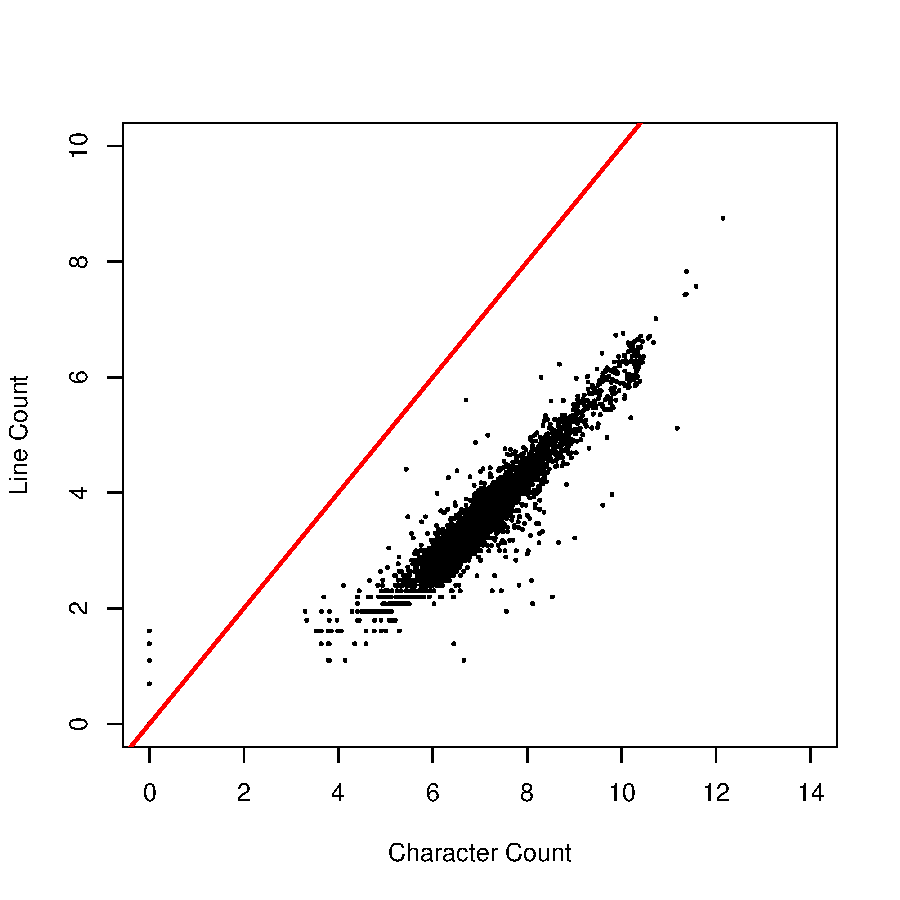
\epsfig{file=Spam/CharVSLineCount,width=10cm}
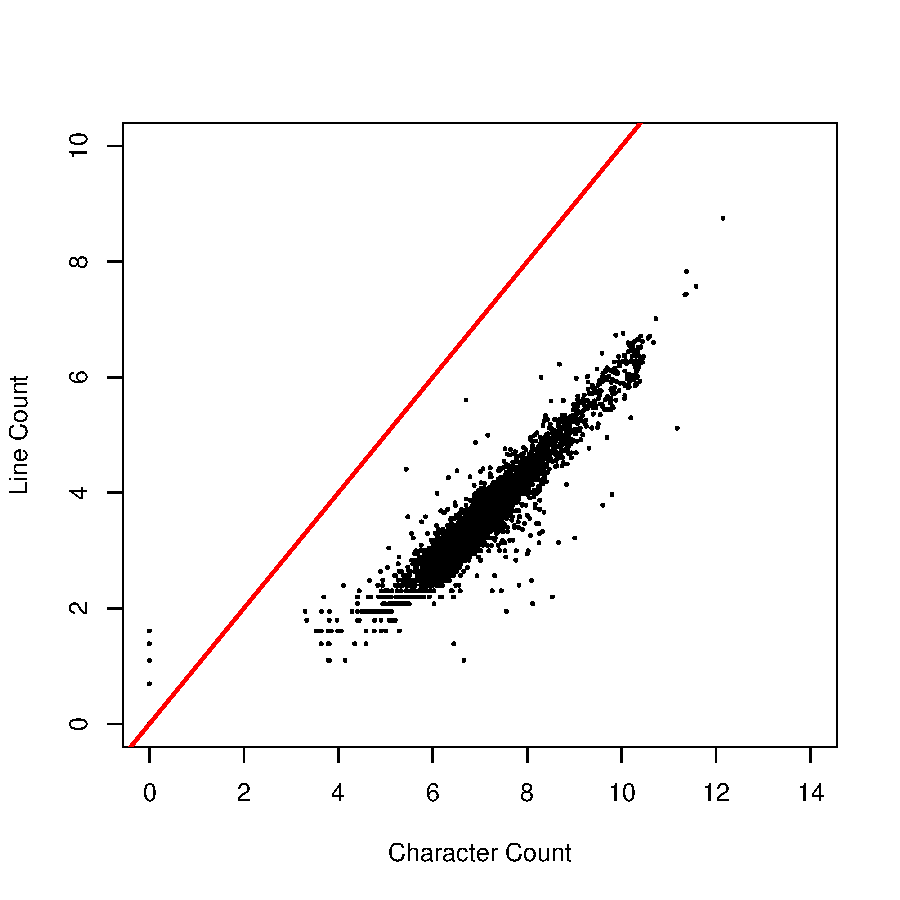
\includegraphics[width=10cm]{Spam/CharVSLineCount.pdf}
\caption{A scatter plot of the number of lines in the 
body of an email message against the number of characters
in the body.  Note that the plot is on log scale, and $1$
is added to all of the values before taking logs.
A few email messages have a few blank lines and nothing
else. These are the only points that fall above the 
$y = x$ red line.}
\label{fig:compareCharLines}
\end{figure}


\subsection{Exploratory Data Analysis}

We derived a few dozen variables from the header, body, and
attachments of each email message. 
Before conducting a formal analysis, we may ask ourselves,
whether or not these derived variables are useful
for predicting spam.
Before embarking on a complex statistical analysis it is
often a good idea to perform some simple analyses to get
a better understanding of the data and its possibilities.
This exploratory analysis may indicate that we need to
do a better job of determing variables from the messages.
This will not only help us in our future statistical
analysis, it will also help us check that the variables
have been correctly coded.

We explore the percentage of capitals in the message body, 
comparing this percentage among spam versus ham messages.  
Side-by-side boxplots (Figure~\ref{fig:boxplotSpam}) help 
us compare the distributions for these two groups.
We see from the boxplots that about 75\% of the ham
data have values at about the lower quartile for the spam
values even though the ham group maximum is much larger
than the spam maximum.  Putting the boxplots on a log
scale makes it easier to make this comparison.
Another way to see this is with a quantile-quantile 
plot. If the two distributions are roughly the same shape
then their paired quantiles will fall on a line.
We see that this is the case for the percent capitals
with spam having a larger mean and greater spread than ham. 
(A slope other than 1 indicates the distributions have
different spread, and an intercept other than zero indicates
a shift in the distributions).

\begin{verbatim}
boxplot(percentCapitals ~ isSpam)
boxplot(log(percentCapitals) ~isSpam)

qqplot(log(percentCapitals[isSpam]),
       log(percentCapitals[!isSpam]))

summary(bodyCharacterCount[isSpam])    
 Min. 1st Qu.  Median    Mean 3rd Qu.    Max.
   0     593    1459    3171    3735   71450

summary(bodyCharacterCount[!isSpam])
 Min. 1st Qu.  Median    Mean 3rd Qu.    Max.
   0     441     883    2290    1567  188500
\end{verbatim}

\begin{figure}
%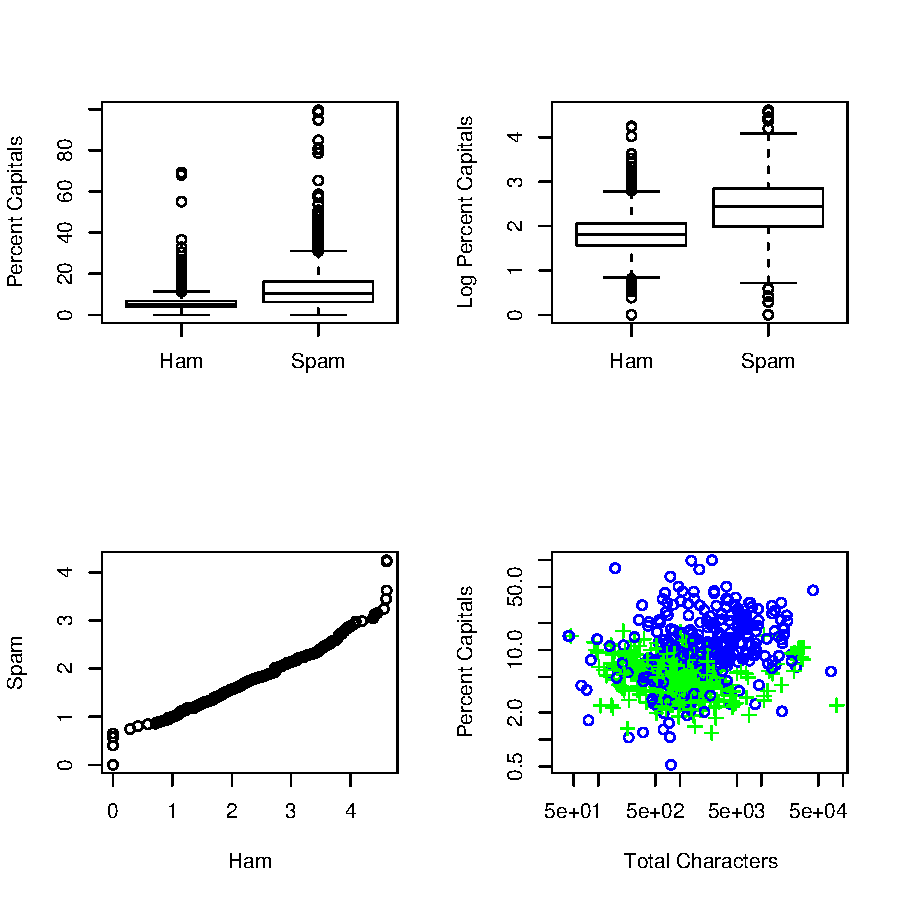
\epsfig{file=Spam/EDApercentCapitals}
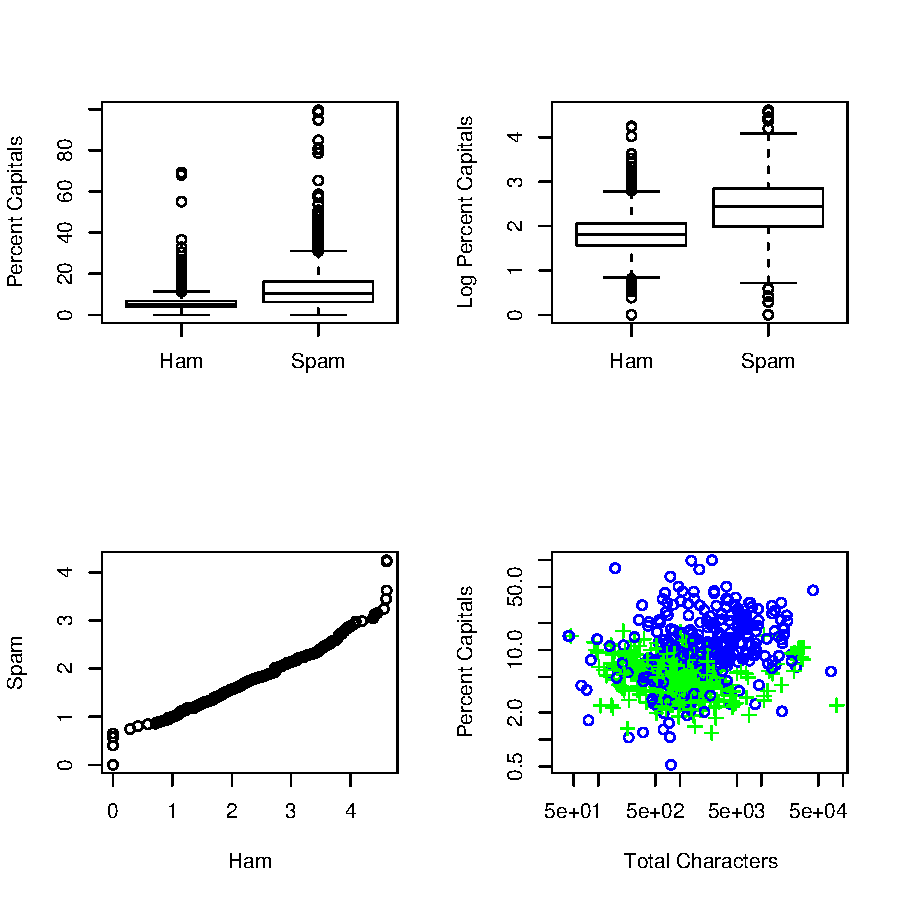
\includegraphics{Spam/EDApercentCapitals.pdf}
\caption{In the two sets of boxplots (top) we see that the 
distribution of the percentage of capitals is skewed with a 
long right tail. 
On a log scale, it is easier to see that about $3/4$ of the spam 
have more capital letters than most of the ham. 
The quantile plot (bottom left) shows that the distribution of capitals
is roughly the same shape for ham and spam.
In the lower right plot, we compare two variables,
percent capitals (crosses) and number of characters (circles)
for 800 randomly sampled emails.}
\label{fig:boxplotSpam}
\end{figure}

Further, we can compare the joint distribution of 
the percentage capitals and the number of characters 
in the body of the message via a scatter plot, 
where the ham is denoted by crosses and the spam by circles.
We see a lot of overlap between ham and spam but the spam
messages tend to be longer and have a greater percentage of capitals.

The numerical summary of the number of attachments (below)
shows that there is very little difference between
spam and ham in that most messages have no attachments.
It is doubtful that this variable will be useful
for classification.
In the two mosaic plots in Figure~\ref{fig:mosiacRe} 
we see that the spam messages are less likely to contain 
an ``Re'' than ham, but more likely to have a numeric end 
to the email address.

\begin{verbatim}
> summary(numAttachments[isSpam])
      Min. 1st Qu.  Median    Mean 3rd Qu.    Max.
    0.0000  0.0000  0.0000  0.2658  0.0000  6.0000
     summary(numAttachments[!isSpam])
     Min.  1st Qu.   Median     Mean  3rd Qu.     Max.
    0.00000  0.00000  0.00000  0.09704  0.00000 19.00000

> par(mfrow=c(1,2))
> mosaicplot(table(isSpam, isRe),shade = TRUE)
> mosaicplot(table(isSpam, fromNumericEnd),shade = TRUE)
\end{verbatim}

\begin{figure}
%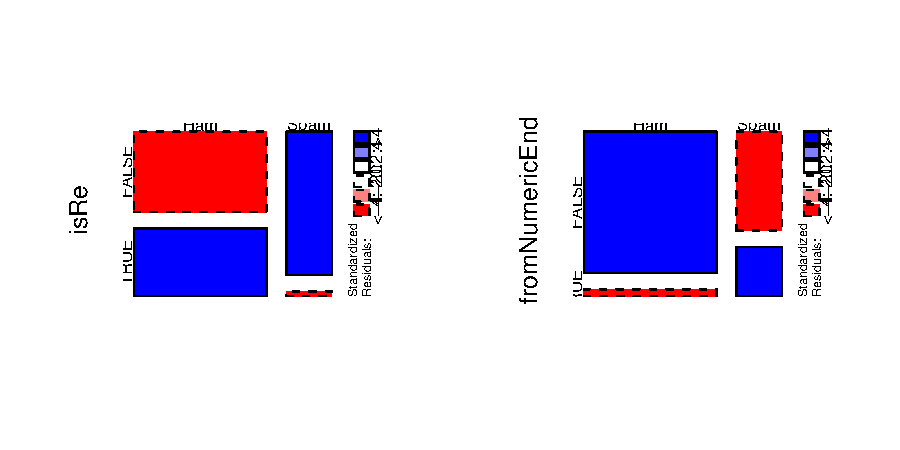
\epsfig{file=Spam/EDAmosaic}
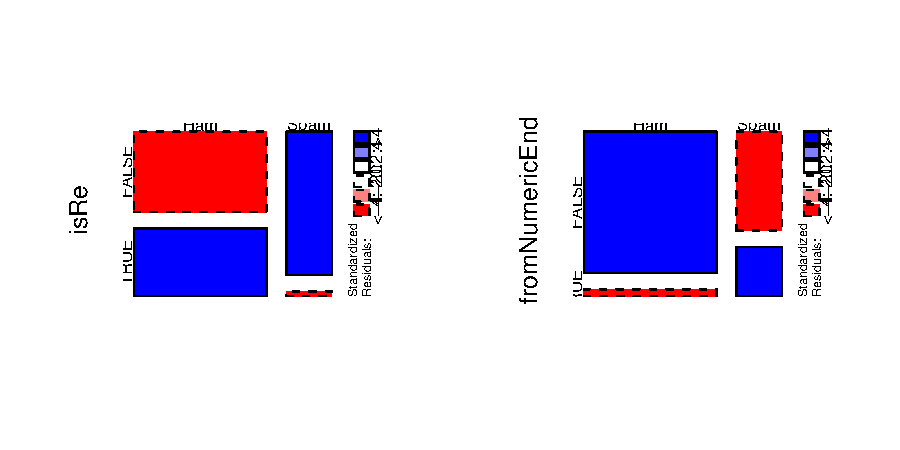
\includegraphics{Spam/EDAmosaic.pdf}
\caption{These two mosaic plots use area to denote 
the proportion of messages that fall in each category.
The plot on the left shows that most of the messages
are ham and have no Re in the subject line.
}
\label{fig:mosiacRe}
\end{figure}


\subsection{Nearest neighbor and Cross-validation algorithms}
Our goal is to create a nearest neighbor classifier to predict whether
a mail message is spam or ham.  To classify an email message, we work
with the variables derived (Section~\ref{sec:derivedVar}) from a
message to find its $k$ nearest neighbors and use them to classify the
message.  A simple classification can be made according to whether the
majority of the $k$ neighbors are spam or ham.  But, we need to
determine $k$.  At one extreme, we have nearest neighbor
classification, when $k$ is $1$, and the new email is classified as
spam or ham depending on whether its nearest neighbor is spam or ham,
respectively.  At the other extreme, we could use all the data
available to us to classify the new email. In this case, the
classification would be the same for any email, i.e. it would be ham
if the majority of the emails in the training set are ham.

To choose a value for $k$, we compare how well the method does for
messages where we know the truth, i.e. when we know whether the new
email is spam or ham.  We can compute the probability that a mistake
is made.  As with the Naive Bayes method in
Section~\ref{sec:naiveBayes}, there are two types of mistakes: a Type
I error occurs when a ham message is incorrectly classified as spam,
and a Type II error when a spam message is misclassified as ham.  We
compare the performance of the $k^{th}$-nearest neighbor classifier
for various values of $k$ via cross-validation to determine the $k$
which best controls these errors.

In the current scenario, we think of our data as pairs $(x_i, y_i)$
for $i= 1, \ldots , n$, where $x_i$ represents the vector of values
for the derived variables from the $i^{th}$ electronic-mail message,
and $y_i$ is an indicator for spam, i.e. it is $1$ when the message is
spam and 0 otherwise.  When a new message comes along we want to use
our nearest neighbor method along with our data to predict whether the
message is spam or ham.  For the new message, we observe the derived
variables, which we call $x_0$, and classify the message as spam if
the majority of its $k$ nearest neighbors among the $\{x_i\}$ are
spam.  For a loss function, ${l}$, the average loss will be

$$  \textbf{E} [ {l}(y_0 , h_k(x_0 ~| ~(x_i , y_i)~ i=1, \ldots , n) )],$$
where $h_k( \cdot ~| ~(x_i , y_i)~ i=1, \ldots , n)$ represents the
nearest-neighbor method that finds the $k$ closest neighbors to $x_0$
among the $x_i$ that are closest to $x_0$ and returns 1 (spam) or 0
(ham) according to whether the corresponding $y_i$ are a majority of
1s or 0s, respectively (Figure~\ref{fig:knnDiagram}).  Zero-one loss,
depending on whether $y_0$ is spam or ham, gives us the desired Type I
and II errors.  As with the Naive Bayes method, we use $v$-fold
cross-validation to approximate this expectation and find the
minimizing $k$.  That is, we divide at random the original data into
$v$ subsets of roughly equal size.  These subsets, $P_1$, $P_2$ ,
$\ldots$, $P_v$ form a random partition of the data.  Then for each
subset, $P_i$, we use $P_i^c$ as the training set:

$$ \frac {1}{v} \sum_{i=1}^v \frac {1} {\#P_i} \sum_{x_j \in P_i} {l}(y_j , h_k(x_j ~|~(x,y) \in P_i^c )) $$
Note that we treat the observations in $P_i$ as new observations and
look for neighbors to these new observations among those in $P_i^c$.
To estimate Type I error we take the average of those $(x_j , y_j)$ in
$P_i$ where $y_j = 0$, and similarly we restrict the average to those
$y_j = 1$ to estimate Type II error.

\begin{figure}

\vspace{2in}

\caption{Diagram of red and green nearest neighbors 
from his lecture notes.}
\label{fig:knnDiagram}
\end{figure}

The above equation helps us understand how cross-validation is
applied to the case of nearest neighbor estimation. It also suggests 
a way to code the nearest neighbor and cross-validation procedures:

\begin{itemize}
\item Partition the data into $v$ subsets.
\item For each observation in a partition $P_i$, 
find the k nearest neighbors in $P_i^c$.
\item Classify the observation according to its neighbors' values. 
\item Repeat for $k = 1, \ldots ,\#P_i^c$
and for $i = 1, \ldots ,v$. 
\end{itemize}

To find the $k$ nearest neighbors, we need to find the distances
between observations. The \Sfunc{dist} function takes a data
frame and computes the distance between all pairs of rows in the data
frame. (For now we ignore the issue of which metric to use and proceed
with the default Euclidean distance).  Although the equation above
provides an intuitive explanation of cross-validation for this
example, it does not indicate an efficient way to program the method.
In this case study, many unnecessary computations can be avoided with
a little attention to the specifics of the problem.  Two important
ones are described here:

\begin{itemize}
\item To find the nearest neighbor in the training set to an
  observation in the validation set, we need to find the distance from
  the validation observation to all observations in the training set.
  But once we have computed all of these distances then we also have
  the $k$ nearest neighbors for $k = 2, \ldots , \#P_i^c$.

\item In one iteration of cross-validation, we need to find the
  distances between all observations in $P_i$ and all those in $P_i^c$
  (Figure~\ref{fig:knnCVdiagram}).  When we consider the iteration
  over $i$, we notice that we need to find distances between all pairs
  of observations because each observation belongs to one validation
  set and $v-1$ training sets.  So, we need only compute all distances
  between pairs of observations in the data once and pull out those
  that are needed for a particular fold $i$ in the $v$-fold
  cross-validation method.
\end{itemize}

\begin{figure}
\vspace{2in}
\caption{Grid figure for cross validating distance matrix}
\label{fig:knnCVdiagram}
\end{figure}

These two properties point out an important feature of 
nearest neighbor methods: no models or parameters are fitted  
that reduce the dimensionality of the problem.
That is, all of the training data must be held around in
order to compute the distance of a new observation to past
observations. 
As a result, for efficiency in terms of space and time,
it is important to take these properties into consideration
when developing the code.
When we do, we see that once we compute all pairs of distances 
between observations, then reordering and subsetting gives us 
all the cross-validated nearest neighbors for any (all) $k$.

The following functions, \SFunctionRef{knnCV} and
\SFunctionRef{knnPredict} take these aspects into consideration.  The
\SFunctionRef{knnPredict} function makes predictions for a test set.
Its inputs are: an $m \times n$ matrix of distances between $m$
observations in the validation and $n$ observations in the training
set; the true classifications for the training set, where spam is
\SValue{TRUE} and ham \SValue{FALSE}; and additional parameters to
specify how to handle ties in voting.  The output is an $m \times p$
matrix of logicals indicating the classification of each element in
the validation set for $p$ different $k$ between \SVariable{kmin} and
\SVariable{kmax}.

The function \SFunctionRef{knnCV} finds the cross-validated prediction
error.  The inputs of this function are: an $N \times N$ matrix of
distances between $N$ observations, the true classification of each of
the $N$ observations, and an $n \times v$ matrix of indices from $1,
..., N$, where the $j^{th}$ column contains the indices $(i_1, \ldots,
i_n) \in \{1, \ldots , N\}$ of the observations in the $j^{th}$
validation set.

\begin{verbatim}
knnCV <-
function(Dist, actualClass, groups, kmin = 1, kmax = 100)
{
# Determine which k's will be reported
  krange  = range(c(kmin, kmax))
  krange[2] = min(krange[2], nrow(groups))  
  knnCorrect = matrix(0, nrow = 0, 
                      ncol = (krange[2] - krange[1] + 1))

 # Loop over v to make predictions for the v test sets
 # using the corresponding v training sets.

  for (i in 1:ncol(groups)) {
    knnPreds = knnPredict( Dist[groups[,i] , - groups[,i]],
                           actualClass[ - groups[, i]], 
                           krange[1], krange[2])

# Determine if the predictions are correct
    knnCorrect = rbind(knnCorrect, 
                   knnCheck( knnPreds, 
                             actualClass[groups[, i]]))
  }

# Compute the Type I and II errors
  ans = predError(knnCorrect, actualClass[groups])
  ans
}
\end{verbatim}

\begin{verbatim}
knnPredict <-
function(distM, trainClass, kmin, kmax, tieRandom = FALSE, 
         tieNearest = FALSE)
{
# distM: m by n matrix where we have m test and 
# n training observations
# trainClass: vector of n logicals

# Returns m by kmax-kmin+1 matrix of logicals (predictions)
  votes <-
      apply(distM, 1, function(nn) {
               tmp = trainClass[order(nn)[1:kmax]]
               percents = cumsum(tmp)/(1:kmax)
               predict = (percents[kmin:kmax] >= .5)
               if (tieRandom) {
                 predict[percents == .5] = 
                    rbinom(n=1,size=1, prob=0.5)
               } else {
                 if  (tieNearest) {
                   predict[percents == .5] = 
                      (percents[1] > 0.5)
                 } else {
                   predict[percents == .5] = 
                      predict[(which(percents == .5) - 1)]
                 }
               } 
               predict  
               })
  t(votes)
}
\end{verbatim}

The computation of the type I and II errors follows the same
approach as shown for the Naive Bayes method so it is not
presented here.


\subsection{Cross-validating the metric}
Now that we have the ability to find type I and type II 
errors for various values of $k$, we turn to the problem
of choosing an appropriate metric for computing distances
between email messages.
One well known metric is Euclidean distance, which 
may not be appropriate for logical variables.
A binary metric may be more appropriate because logicals
take on only two possible values.  
For variables, such as the number of lines in the
body of the email \SVariable{numLinesInBody}, 
the percentage of capital letters in the subject of the email
\SVariable{percentCapitals}, 
and the number of recipients \SVariable{numRecipients},
we compute the Euclidean distance between two email
messages $i$ and $j$ as follows:
\begin{eqnarray*}
 [(numLinesInBody_i &-& numLinesInBody_j)^2 \\
   &+& (percentCapitals_i - percentCapitals_j)^2\\
     &+& (numRecipients_i - numRecipients_j)^2 ]^{1/2} 
\end{eqnarray*}
and the Manhattan distance between them is:
\begin{eqnarray*}
  |numLinesInBody_i &-& numLinesInBody_j|\\
    &+& |percentCapitals_i - percentCapitals_j|\\
      &+& |numRecipients_i - numRecipients_j|
\end{eqnarray*}

Note however that the percentage of capitals in the subject will always
be between 0 and 100, whereas the number of lines in the body of an
email can get quite large.
We may want to normalize the continuous variables before
computing the distance between two records.
One way to do this is center the variable on
the mean value and to scale it by the standard deviation,
i.e.
$$
\frac{(numLinesInBody - mean(numLinesInBody))}
{SD(numLinesInBody)} .$$
Alternatively, the median and median asolute deviation could
standardize a variable.
Or, proportions and percentages (scaled by 100) could be left
alone, and the other non-binary values scaled by 3SDs to bring
them all in the range of 0 to 1. 
The Canberra distance includes a standardization,
\begin{eqnarray*}
 &~& \frac {|numLinesInBody_i - numLinesInBody_j|} 
  {|numLinesInBody_i + numLinesInBody_j|} \\
    &+& \frac {|percentCapitals_i - percentCapitals_j|} 
            {|percentCapitals_i + percentCapitals_j|} \\
      &+& \frac {|numRecipients_i - numRecipients_j|} 
            {|numRecipients_i + numRecipients_j|}
\end{eqnarray*}

The rule for the asymmetric distance is as follows:
compute the number of elements in the vectors for which at least one
of the two records has a non-zero value; count the number of these
elements for which the two records are different (i.e. one is a 1
and the other is a 0); and report the proportion of these two
counts as the distance.  
When neither record has any 1s, the distance is 0.
An example may help. Suppose we look the three variables
\SVariable{isRe}, \SVariable{replyUnderline} and \SVariable{multipartText}
and we have email records $i$ and $j$ as

\begin{verbatim}
    isRe    replyUnderline   multipartText
    TRUE          FALSE         FALSE
    FALSE         FALSE         FALSE
\end{verbatim}
The distance is 1 (or 1/1) since there is only one
entry for which there is at least one 1 (i.e. TRUE).
And in this position (the first), the values are different so we count 1.
For two records of the form
\begin{verbatim}
     isRe    replyUnderline   multipartText
     TRUE        TRUE            TRUE
     FALSE       FALSE           TRUE
\end{verbatim}
the distance would be 2/3.

Whichever metric we use, we then have to combine the distance 
values, $D$, for the binary and non-binary variables. 
An obvious way to combine them is
\[ D_{\textrm{non-binary}} + w D_{\textrm{binary}}\]
Of course, we need to determine $w$, so we use cross-validation
to obtain values for both $w$ and $k$.

Since we have our cross-validation functions for finding $k$, 
we can write a simple wrapper function to cross-validate the metric
and the weight $w$.
The function \Sfunc{knnExpr} takes various values of these
three parameters ($k$, $w$, and the metric) and cross-validates the
prediction error for all combinations of the values.  
The R function
\Sfunc{dist} computes distances via various metrics,
including Euclidean, Manhattan, Minkowski, Canberra, 
and asymmetric binary.

\begin{verbatim}
knnExpt <-
function(derivedEmails, actualClass, w = 1, 
         metric = c("euclidean", "manhattan", "canberra"), v = 10, 
                    perm = sample(1:nrow(derivedEmails)),
                    kmin = 1, kmax = 100)
{
   logVars = which(sapply(derivedEmails, is.logical))
   conVars = (1:ncol(derivedEmails))[-logVars]

   binDist = as.matrix(dist(derivedEmails[, logVars], 
                            method = "binary"))
   groups = cvSet(v = v, perm = perm) 

   for(i in metric) {
      conDist = as.matrix(dist(derivedEmails[, conVars],
                               method= i))
      predErrs = list()
      for (j in 1:length(w)) 
        {
           Dist = (w[j] * binDist) + conDist
           predErrs[[j]] = knnCV(Dist, actualClass,   
                                 groups, kmin, kmax)
           remove(Dist)
        }
      assign(paste("outKNN", i, sep = "."), predErrors)
      save(paste("outKNN", i, sep = "."), 
           file =paste("outKNN", i, ".rda", sep = ""))
    }
}
\end{verbatim}
Note that we use the \Sfunc{assign} function here 
in order to create an R object with name based on the metric
specified via an input parameter at the time the function is called. 

We use the following script to analyzes the email messages.
It takes the default values for the metrics (Canberra, Manhattan,
and Euclidean) and for the $k$ (1 to 100), and specifies $w$ only.
We may want to run the script in batch mode (say more ...).
The script is annotated to explain the various steps of the 
analysis process.

\begin{verbatim}
# All of the functions are in the file myKNN.S.
source("myKNN.S")
# Load the data to cross-validate
load("knnData.rda")

# After exploratory data analysis we settle on transforming
# the non-binary variables which are also not proportions/percentages

logTrans = c("numLinesInBody", "numAttachments", 
             "numRecipients", "numDollarSigns", 
             "bodyCharacterCount", "subjectQuestCount",
             "subjectExclamationCount", "averageWordLength")

for (i in logTrans) {
    derivedEmails[, i ] = log(1+ derivedEmails[, i])
}
# Transform the time to fall between 0 and 1.
derivedEmails[,"hourSent"]= derivedEmails[,"hourSent"]/24

actualClass = derivedEmails[, "isSpam"]
knnExpt(derivedEmails, actualClass, w = c(1,5,10,15,20))
\end{verbatim}

Once we have the cross-validated prediction errors, plots such as those
in Figure~\ref{fig:knn1to100} show us that the metrics produce similar
results, with Manhattan and Canberra slightly outperforming Euclidean.
We make the following observations.

\begin{figure}
%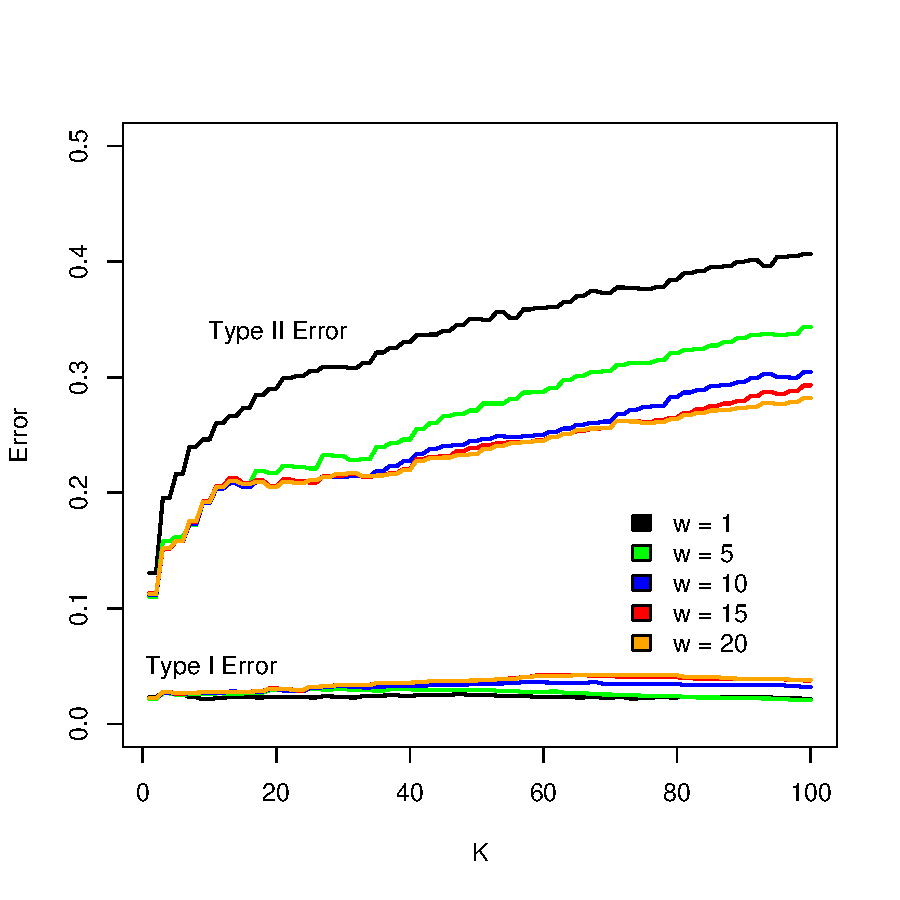
\epsfig{file=Spam/knn1to100}
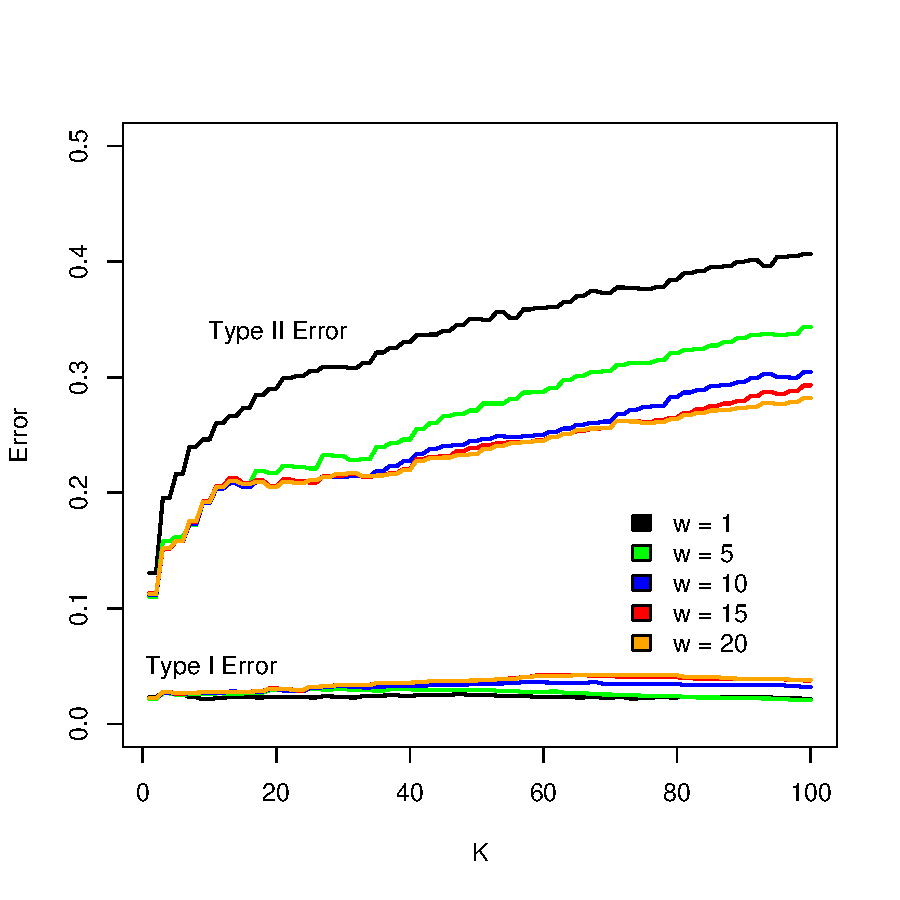
\includegraphics{Spam/knn1to100.pdf}
\caption{Type I and II error rates for Canberra distance.}
\label{fig:knn1to100}
\end{figure}

\begin{itemize}
\item The Type I error is much smaller than Type II, and has less variability.

\item There is a sharp increase in Type II errors as $k$ grows, and we need to
zoom in on the region where $k< 15$ in order to see better which value of 
$w$ should be used (Figure~\ref{fig:knn1to15}).

\begin{figure}
%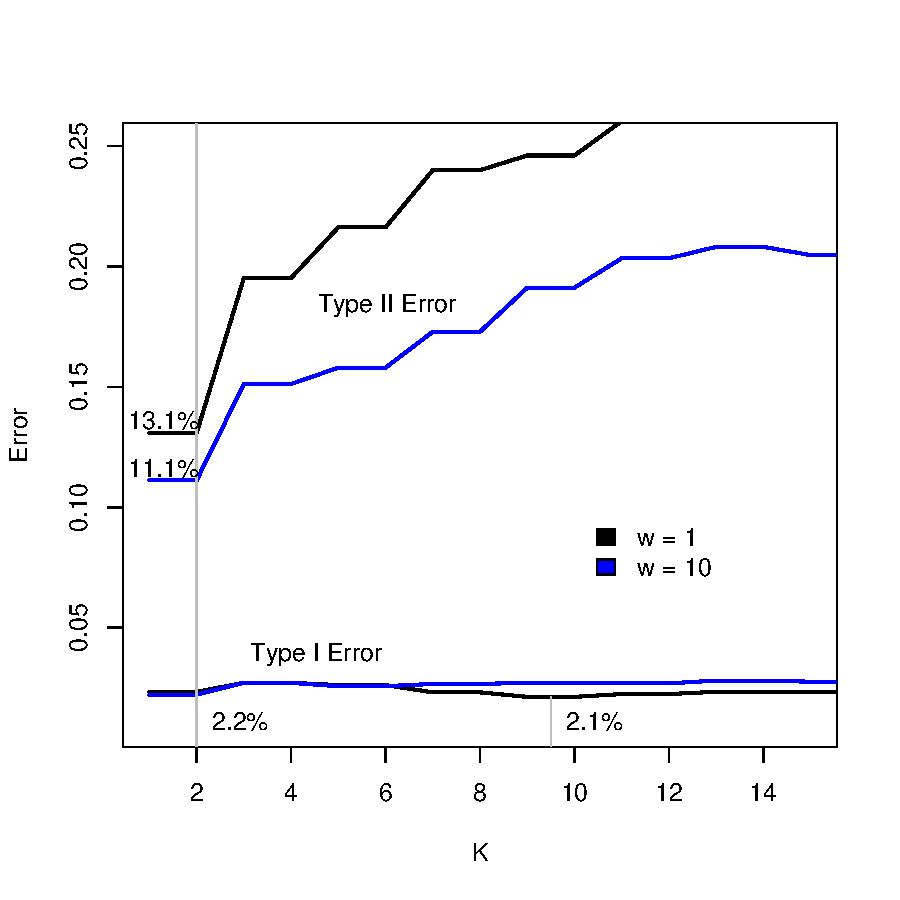
\epsfig{file=Spam/knn1to15}
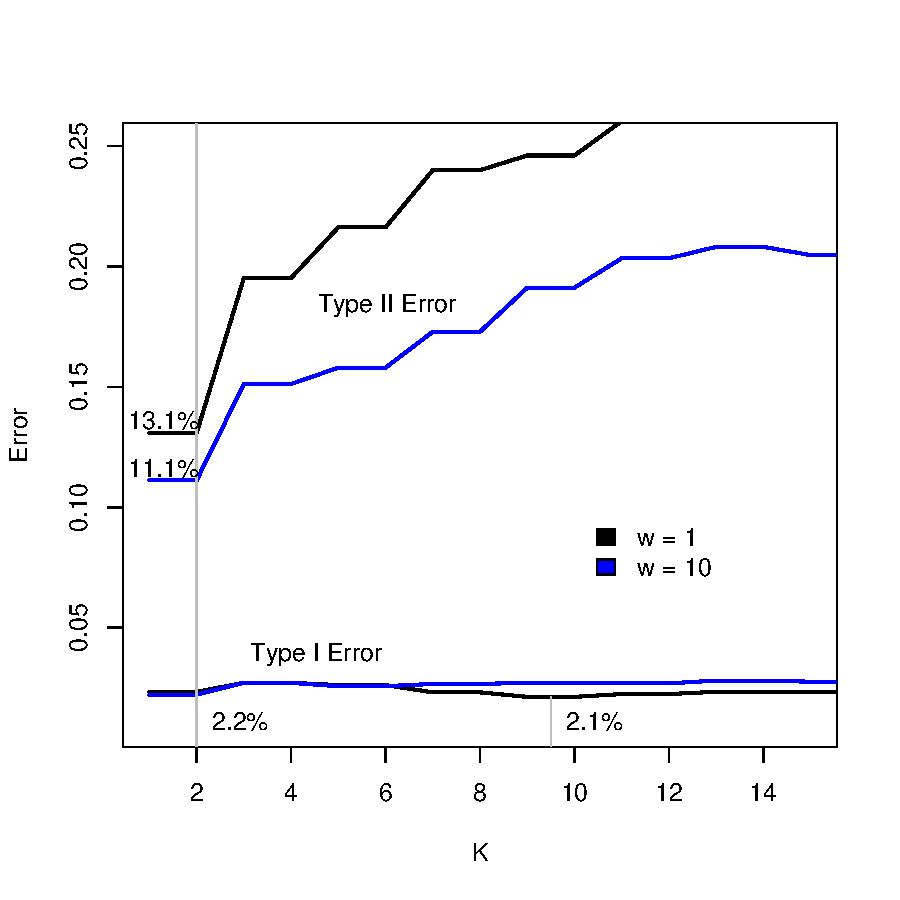
\includegraphics{Spam/knn1to15.pdf}
\caption{Type I and II error rates for Canberra distance.}
\label{fig:knn1to15}
\end{figure}

\item The Type II error is minimized at $k=1, 2$, regardless of the value for $w$,
but it does appear that there is a big drop in the Type II errors for larger weights.
In order to see which weights do best, we need to zoom in on the Type II errors 
separately because they are on a different scale in comparison to Type I errors
(Figure~\ref{fig:knnTypeII}).
In this figure, we see that the curves for Type II error
are the same shape with w=10 being the best.

\item Similarly, we see that for Type I (Figure~\ref{fig:knnTypeI}), 
when $w=1$, the best $k$ is about $9$, with $k=1,2$ a close second. 
For $w = 1$, the Type I error curve has a sharp dip at the minimum
and slowly rises for larger $k$, but remains relatively small in
comparison to the Type II error for all $w$..
\end{itemize}

Based on these considerations, we choose $k = 2$, $w = 10$, and the 
Canberra metric.

\begin{figure}
%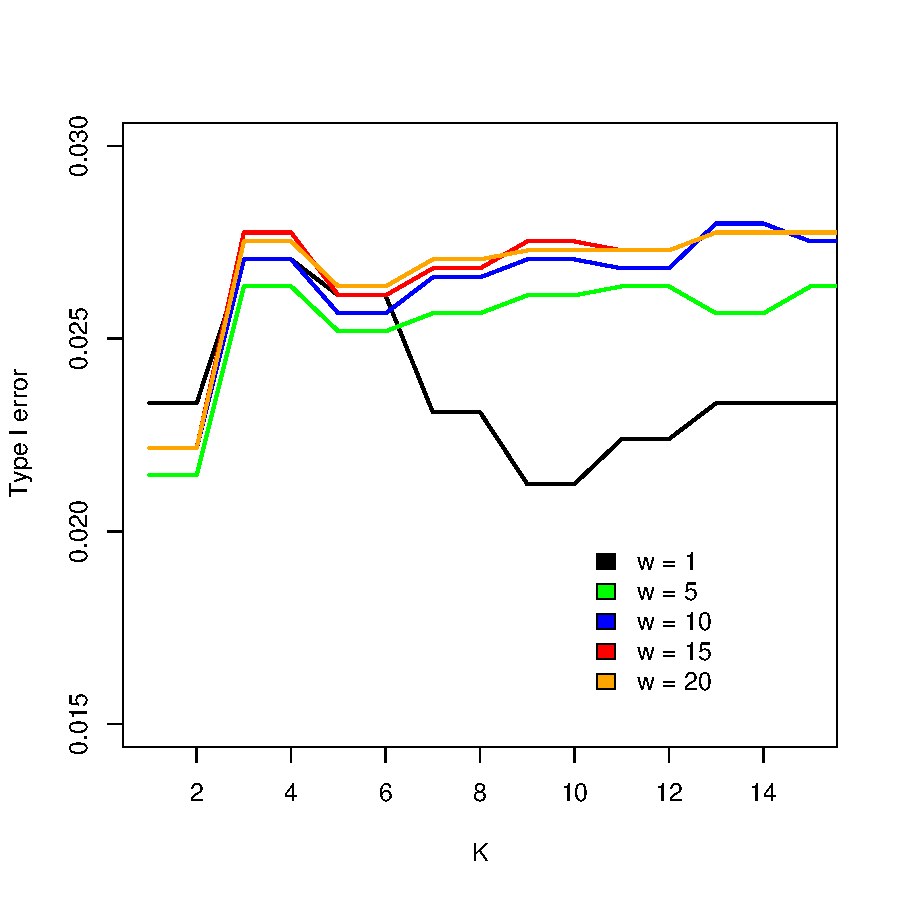
\epsfig{file=Spam/knnTypeI}
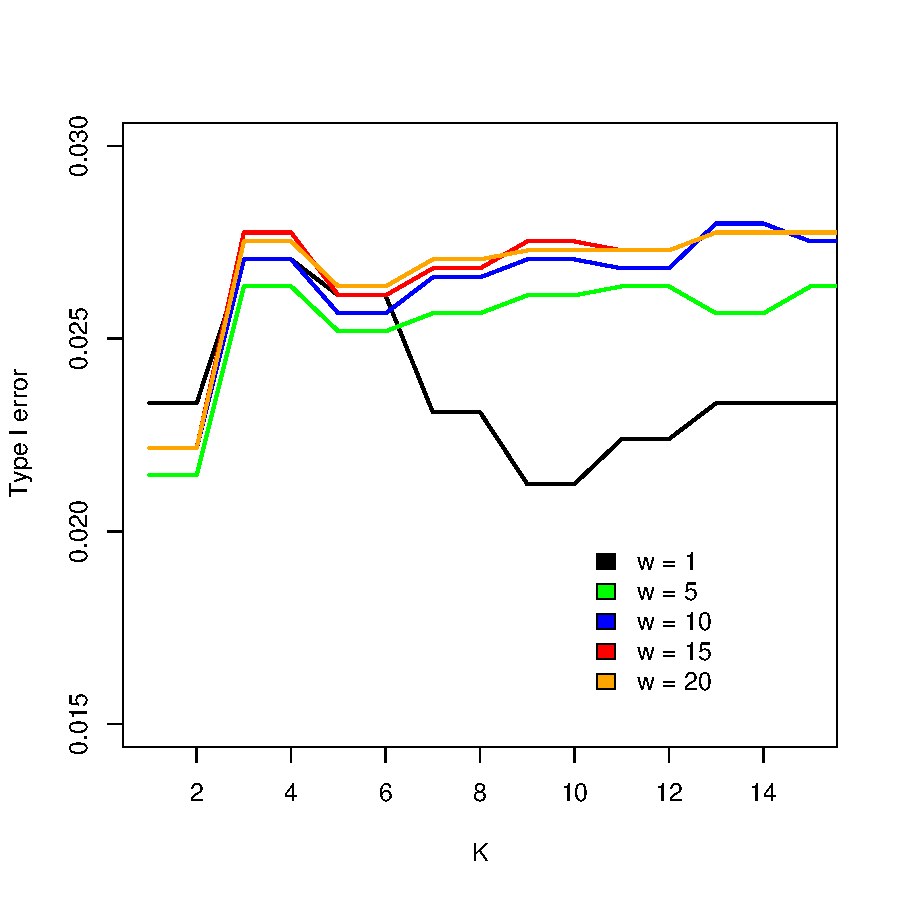
\includegraphics{Spam/knnTypeI.pdf}
\caption{Type I error rates for Canberra distance.}
\label{fig:knnTypeI}
\end{figure}

\begin{figure}
%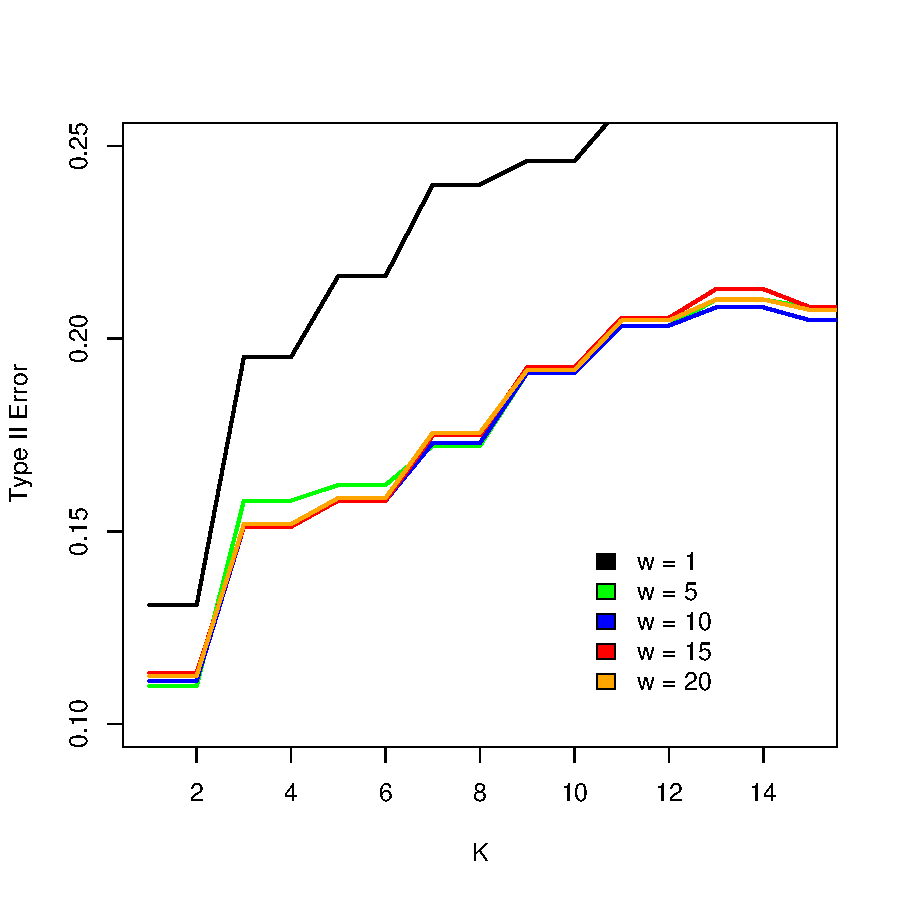
\epsfig{file=Spam/knnTypeII}
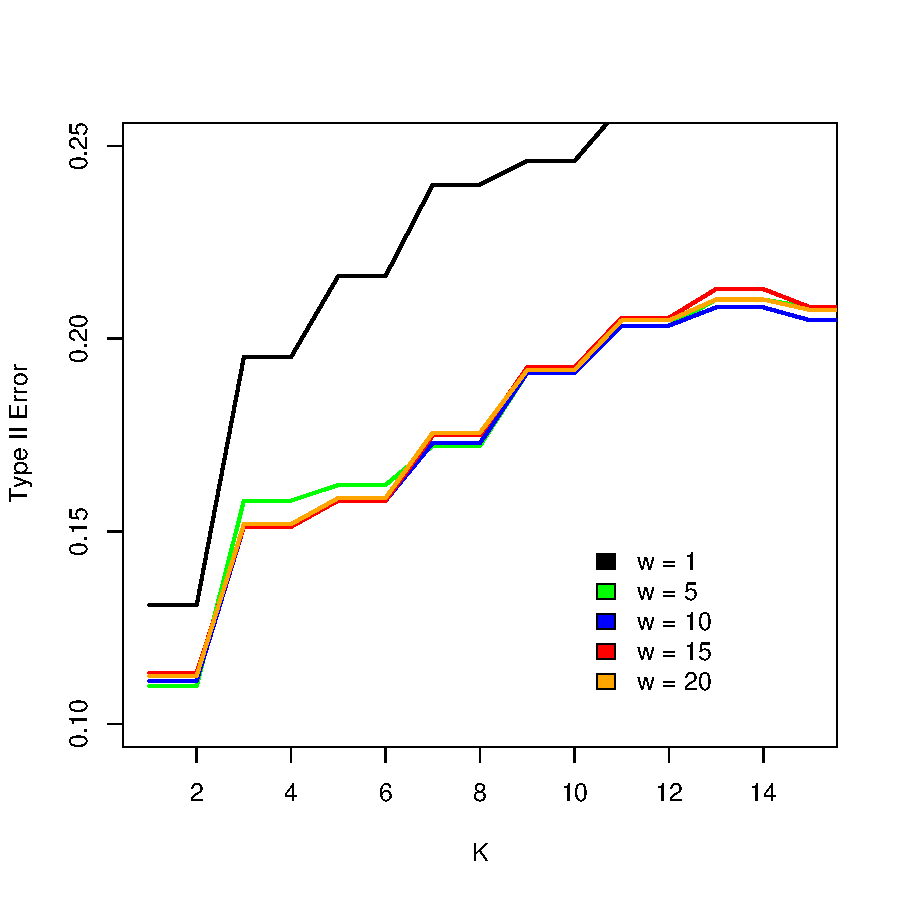
\includegraphics{Spam/knnTypeII.pdf}
\caption{Type II error rates for Canberra distance.}
\label{fig:knnTypeII}
\end{figure}


\subsection{Further validation and comparison}
We can validate how well $k^{th}$ nearest neighbor
performs on a new, independent set of date.
We mean here validate, not cross-validate, because
we have set aside a portion of the Spam Assassin data for 
this purpose, and did not use it to select
the parameters, $k$, $w$ and the non-binary metric.
We now apply the nearest-neighbor method to these
new data, with $k =2$, $w = 10$, and the Canberra metric,
and compute the Type I and II errors.

We reap the benefits now of having written separate functions
for the two distinct tasks: classification and  cross-validation.
We do not have to write additional code in order to apply
the classification to the new data.
We need only prepare the data for inputting to our function.
We first construct the distance matrix from the combined data,
i.e. the original set, \SVariable{derivedEmails} and the
new validation set of 750 messages, \SVariable{newEmails}.
Then we use \Sfunc{knnPredict} to make the
nearest neighbor predictions, where a prediction is made
for each message in \SVariable{newEmails} by looking
for neighbors among the observations in \SVariable{derivedEmails}.

\begin{verbatim}
testEmails = rbind(derivedEmails,newEmails)
nOld = nrow(derivedEmails)

binDist = as.matrix(dist(testEmails[, logVars], 
                         method = "binary"))
conDist = as.matrix(dist(testEmails[, conVars], 
                         method = "canberra"))
bothDist = (10*binDist) + conDist
remove(binDist,conDist)

actualClass = testEmails[,1]
knnPreds = knnPredict(bothDist[ -(1:nOld), 1:nOld],
              actualClass[1:nOld], kmin = 1, kmax = 10)
knnCorrect = knnCheck(knnPreds, actualClass[-(1:nOld)])
knnErrs = predError(knnCorrect, actualClass[-(1:nOld)])
\end{verbatim}

We find that both Type I and II errors are worse for these
750 new observations (they are both over 17\%).
Why did the method not work as well on these observations?
There may be a difference between the data that have been
held out and the data that we used to choose $k$ and $w$.

Exploratory analysis of the data reveals several
differences between the old and new mail messages.
These are presented in tables below.
We see that there is little difference between
the two sets of email messages in terms of the presence
of ``Dear'' in the email, \SVariable{isDear}; and
there is a small difference between old and new
as far as the amount of yelling in the subject line,
\SVariable{isYelling}. 
But there is a big difference in the use of ``Re'';
75\% of the new ham has an ``Re'', in comparison to 57\% 
of the old ham.
Also, there is a large difference when it comes to the
use of a numeric end on the email address. 
Less than 5\% of the old ham has a numeric end in comparison 
to 22\% of new ham, and roughly 30\% of spam whether old or new 
has a numeric end.

\begin{table}
\begin{tabular}{rrrrrr}
       &  &  \multicolumn{2}{c}{Old Mail} & \multicolumn{2}{c}{New Mail} \\
       & isDear & FALSE & TRUE & FALSE & TRUE \\
isSpam & FALSE & 4287  &   0  & 500 &  0\\
       & TRUE  & 1380  &  44 & 237 & 7 \\
\end{tabular}
\end{table}

\begin{table}
\begin{tabular}{rrrrrr}
       &  &  \multicolumn{2}{c}{Old Mail} & \multicolumn{2}{c}{New Mail} \\
       & isYelling & FALSE & TRUE & FALSE & TRUE \\
isSpam & FALSE & 4278  &   6  & 493 &  4\\
       & TRUE  & 1346  &  129 & 234 & 16 \\
\end{tabular}
\end{table}

\begin{table}
\begin{tabular}{rrrrrr}
       &  &  \multicolumn{2}{c}{Old Mail} & \multicolumn{2}{c}{New Mail} \\
       & isRe & FALSE & TRUE & FALSE & TRUE \\
isSpam & FALSE & 2459  & 1828 & 376 & 124\\
       & TRUE  & 1432  &  43  & 245 &  5 \\
\end{tabular}
\end{table}

\begin{table}
\begin{tabular}{rrrrrr}
       &  &  \multicolumn{2}{c}{Old Mail} & \multicolumn{2}{c}{New Mail} \\
       & fromNumericEnd & FALSE & TRUE & FALSE & TRUE \\
isSpam & FALSE & 4085  & 202  & 392  & 108 \\
       & TRUE  & 984  &  491  & 175 &  75  \\
\end{tabular}
\end{table}

The boxplots on a log scale show that: the
number of characters in the message body for the 
new ham has a long left tail (Figure~\ref{fig:knnBoxPlotBCC})
and so will more likely be confused with the old spam;
the proportion of capital letters to all letters in the
body of the message and the proportion of blanks in the 
subject line both appear about the same
in the new and old emails (Figures~\ref{fig:knnBoxPlotPC}
and~\ref{fig:knnBoxPlotPSB});
but there are far more forwards in the old ham than in
the new ham. 

\begin{figure}
%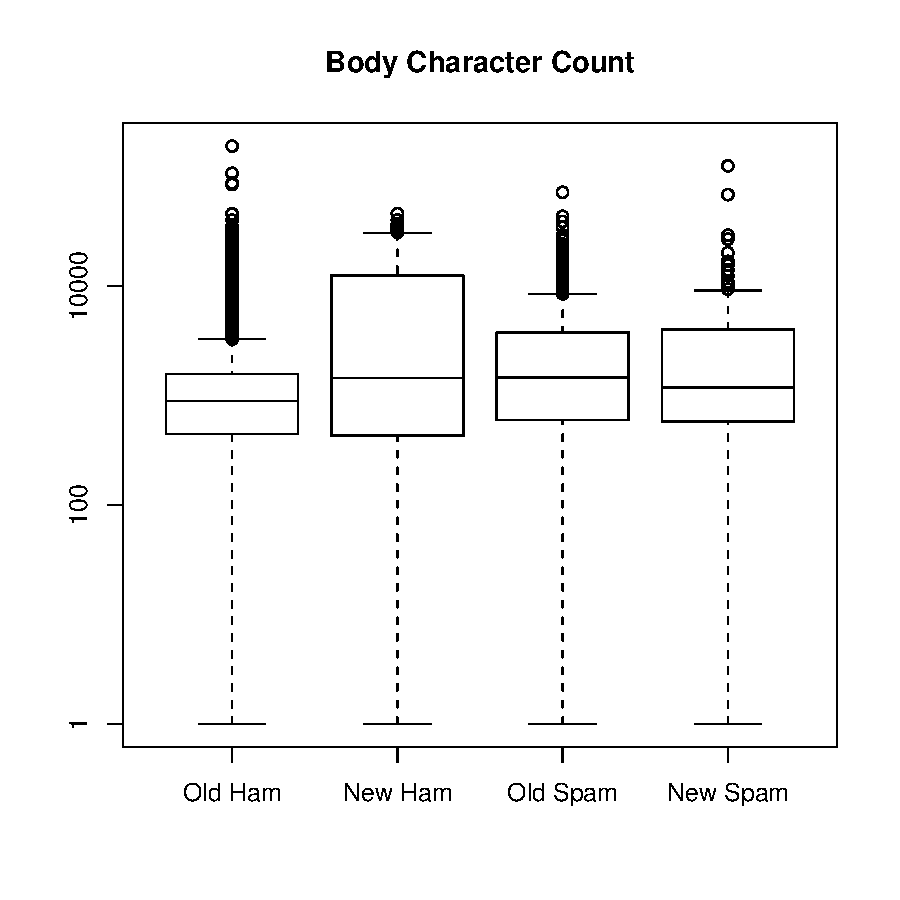
\epsfig{file=Spam/knnBoxPlotBCC}
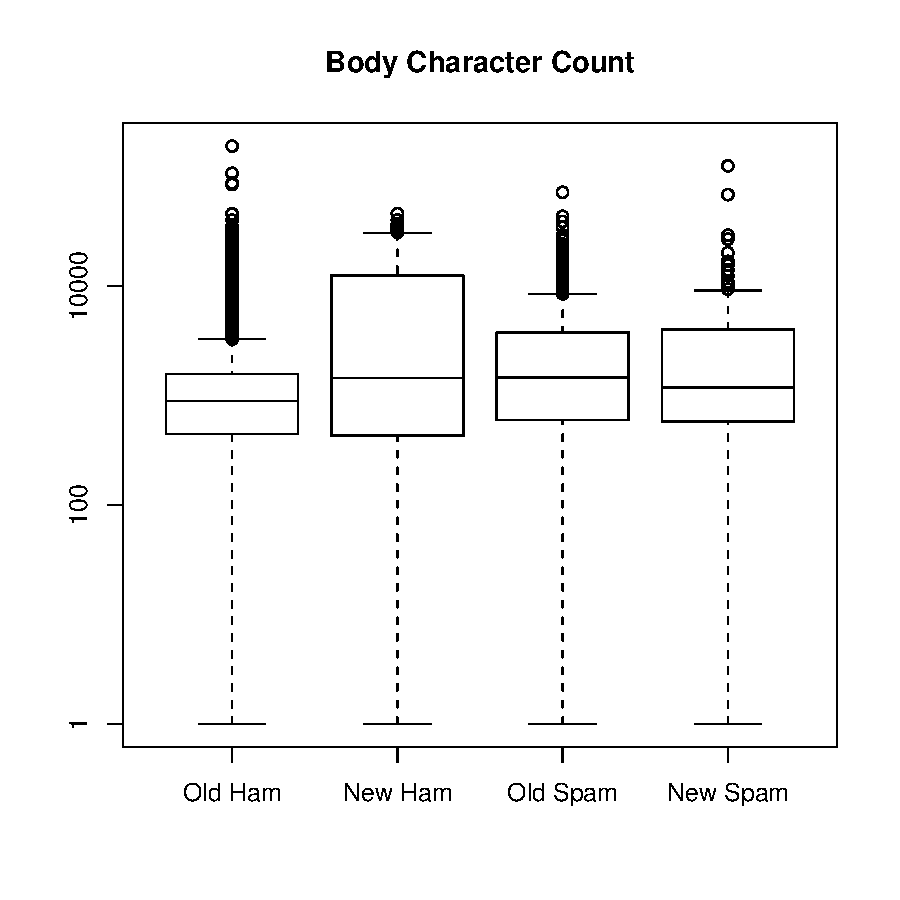
\includegraphics{Spam/knnBoxPlotBCC.pdf}
\caption{Boxplot of the number of characters in the body of the
email message. The counts are one a log scale.}
\label{fig:knnBoxPlotBCC}
\end{figure}

\begin{figure}
%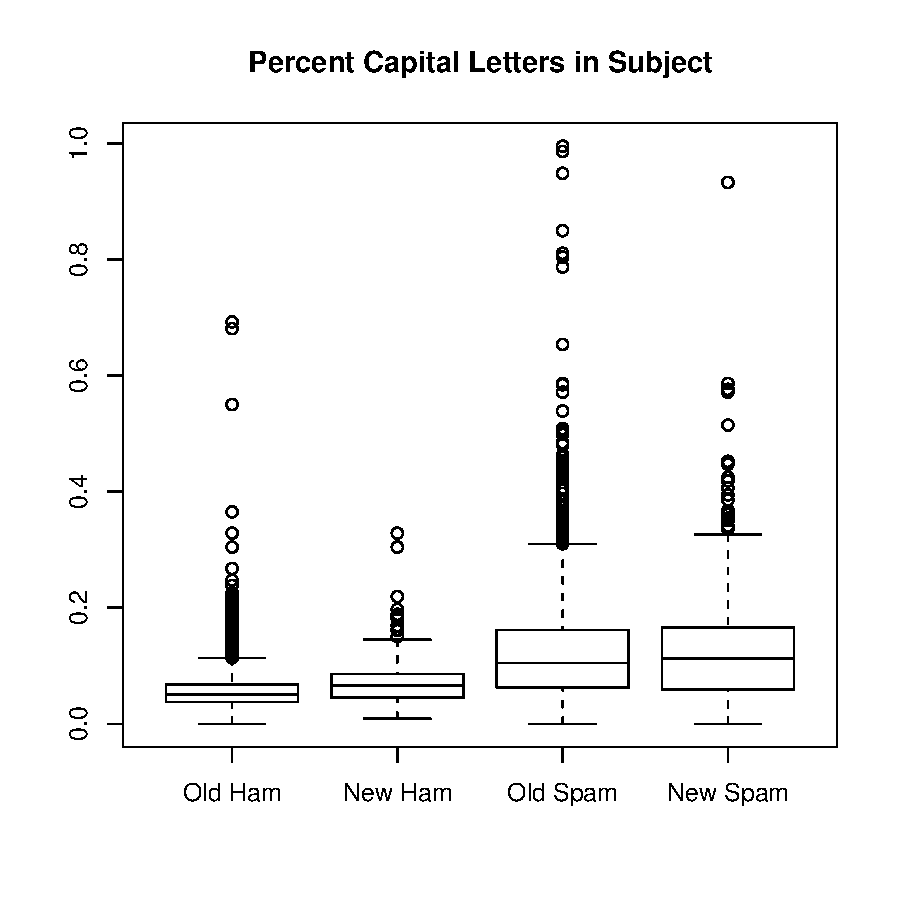
\epsfig{file=Spam/knnBoxPlotPC}
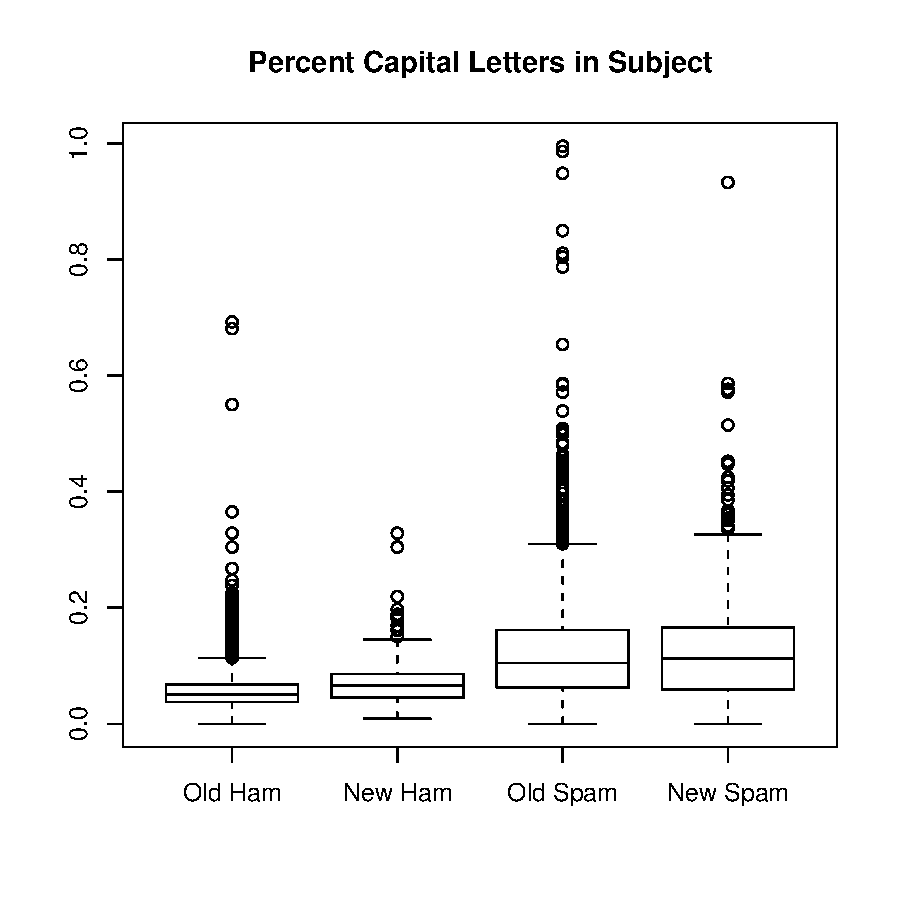
\includegraphics{Spam/knnBoxPlotPC.pdf}
\caption{Boxplot of the percenatge of characters in the body which
are capitalized. The percentage is one a log scale.}
\label{fig:knnBoxPlotPC}
\end{figure}

\begin{figure}
%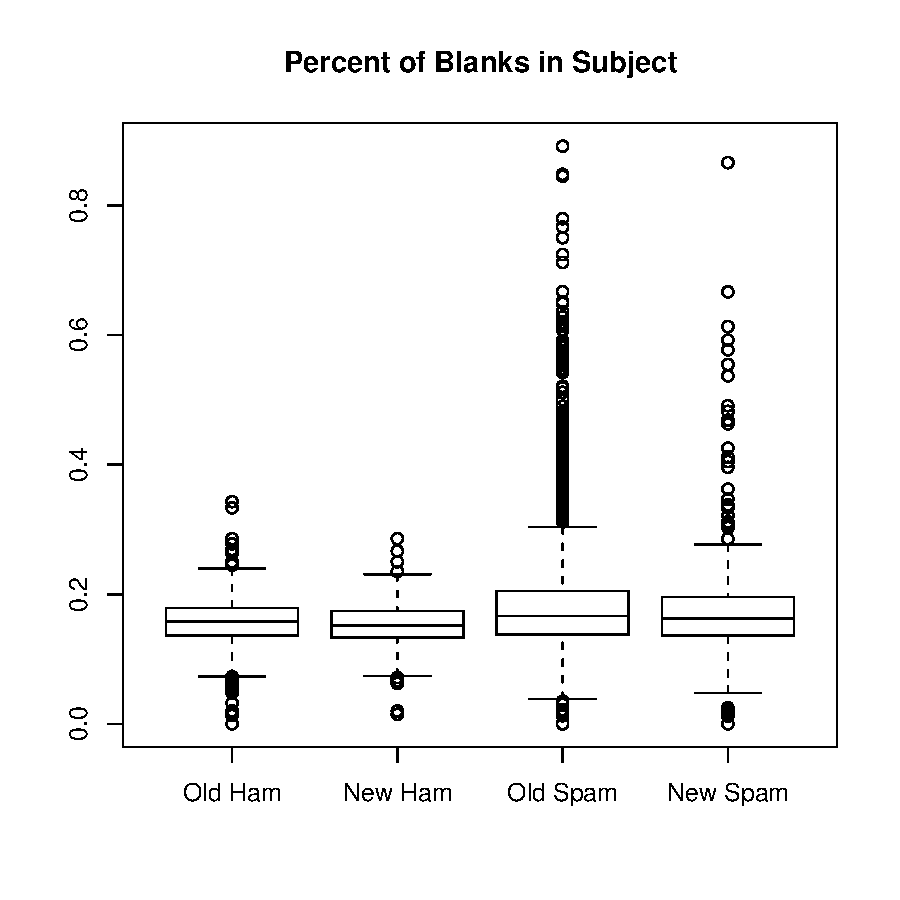
\epsfig{file=Spam/knnBoxPlotPSB}
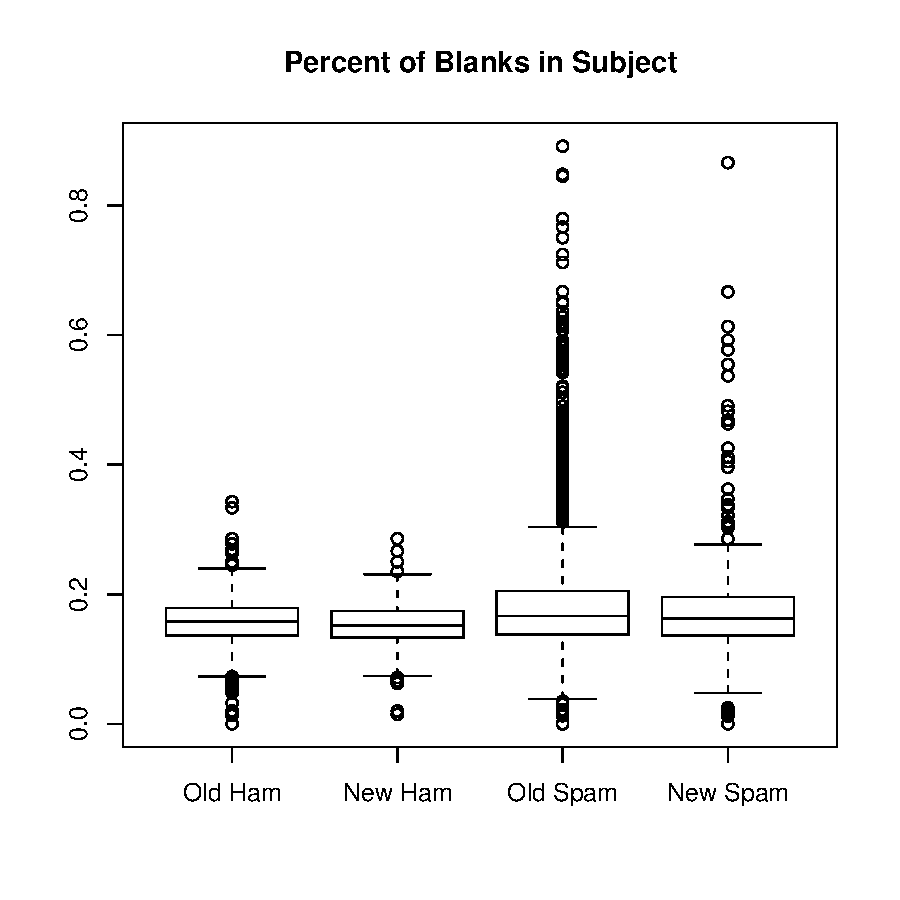
\includegraphics{Spam/knnBoxPlotPSB.pdf}
\caption{Boxplot of the percentage of blanks in the subject line.
The percentage is one a log scale.}
\label{fig:knnBoxPlotPSB}
\end{figure}


We complete the chapter by comparing our optimal nearest neighbor 
procedure to the method of classification trees.
A classification tree is an intuitively simple classification
method. Beginning at the root node of the tree, the data
split or branch into two groups according to the
value of a single variable.
For example, the first split in the classification tree shown in
Figure~\ref{fig:rpartTree} is according to the value of 
percentCapitals, where the data are divided into two groups
according to whether an observation's value for percentCapitals is
above $0.1136$ or not. 

\begin{figure}
%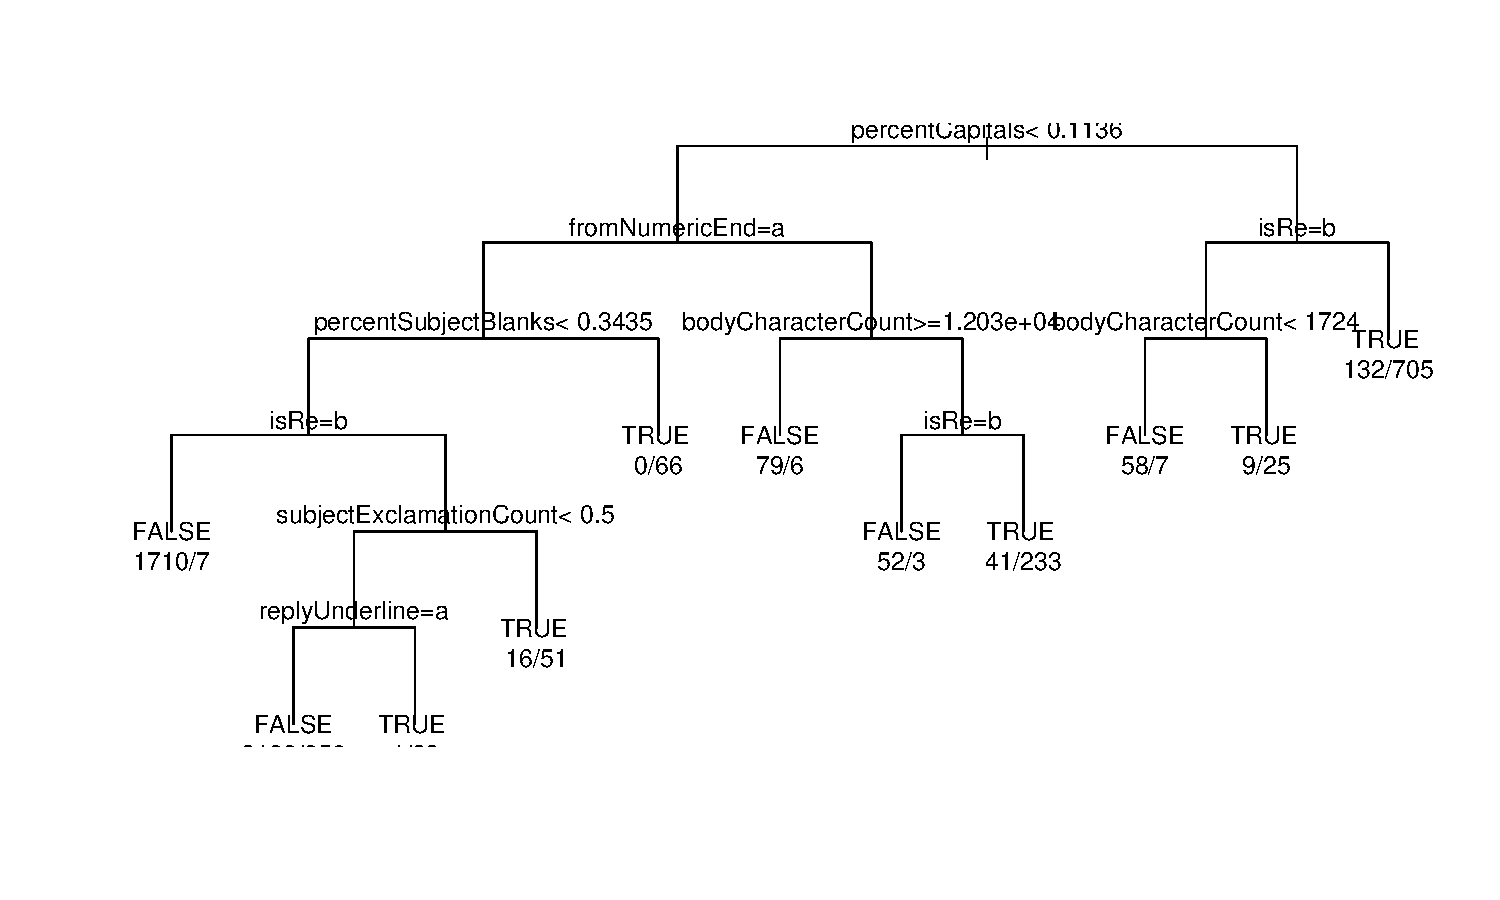
\epsfig{file=Spam/rpartTree, angle=90, height=8in}
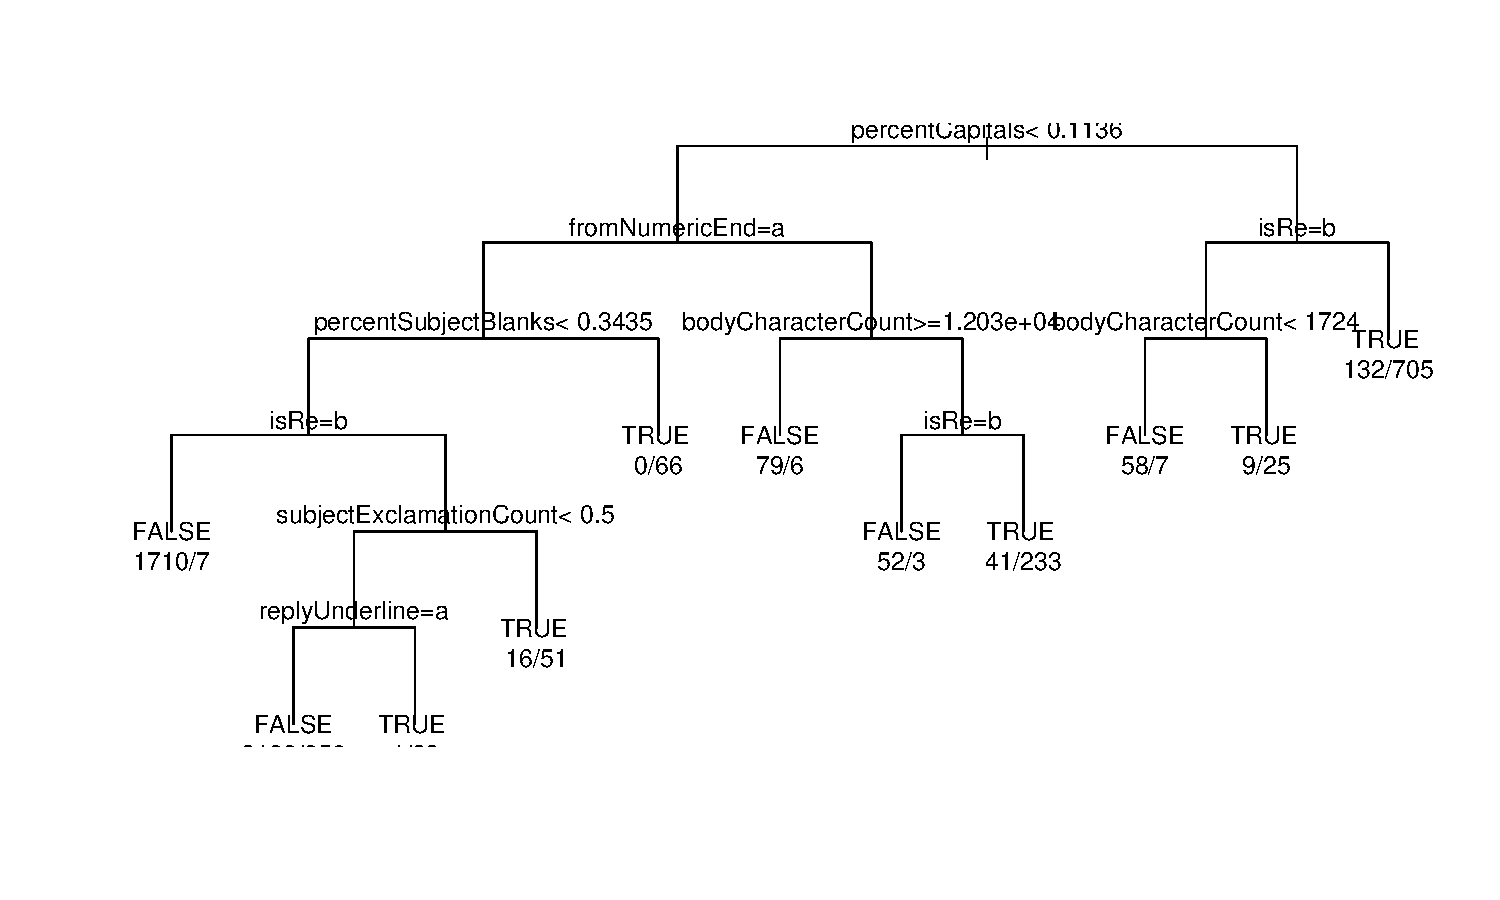
\includegraphics[height=6in, angle=90]{Spam/rpartTree.pdf}
\caption{Classification tree for spam built using the
default arguments to \Sfunc{rpart}}
\label{fig:rpartTree}
\end{figure}

Subsequent splits are made along the resulting two branches
in a similiar fashion; that is, each split considers the
value of a single variable and subdivides the 
data at that node into two groups according to whether the
observation falls above or below the chosen value. 
The variables must all be either factors or numeric.
For a factor variable, the split is made according to a 
particular level of the factor; that is, if an observation has 
that particular factor level than it branches to the right,
otherwise it branches to the left.

The branching attempts to make the observations in the resulting 
subgroups as similar as possible. 
All observations in a subgroup 
at the end of the tree (i.e. a leaf) are given the same classification.
If the observations in the leaves are as homogeneous as possible, 
then we reduce the prediction error.
Does the classification tree approach outperform 
the nearest neighbor approach?
We use the \SPackage{rpart} package to build a classification
tree using the original data in \SVariable{derivedEmails}, 
and then we evaluate the tree's predictive abililty on 
the new set of emails messages in \SVariable{newEmails}.

Before we proceed, we investigate how to use the 
\SPackage{rpart} package.
The \Sfunc{rpart} function returns an object of class
\SClass{rpart}, which means that many functions
know how to handle this object. 
For example, if we use the \Sfunc{plot} function 
with an \SClass{rpart} object,
it will plot the subdivisions of the data as a tree. 
That is how the trees in Figures~\ref{fig:rpartTree}
and~\ref{fig:repartTree00001} are made, with simple
calls to the \Sfunc{plot} function.
Also, the \Sfunc{predict} function (see help
on \Sfunc{predict.rpart} allows us to 
classify records using an \SClass{rpart} object.
To find out more about the \SPackage{rpart}
library, read the documentation at\\
\texttt{http://cran.r-project.org/doc/packages/rpart.pdf}\\
or other documentation that you may find in a Google search.

\begin{comment}
\begin{figure}
%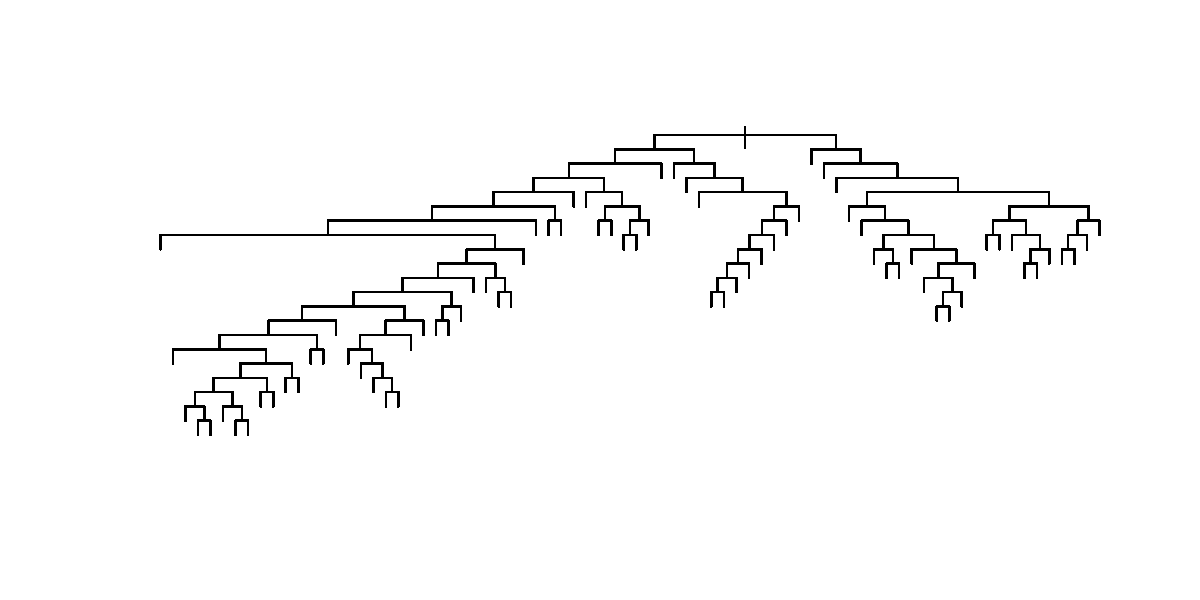
\epsfig{file=Spam/rpartTree00001, angle =90}
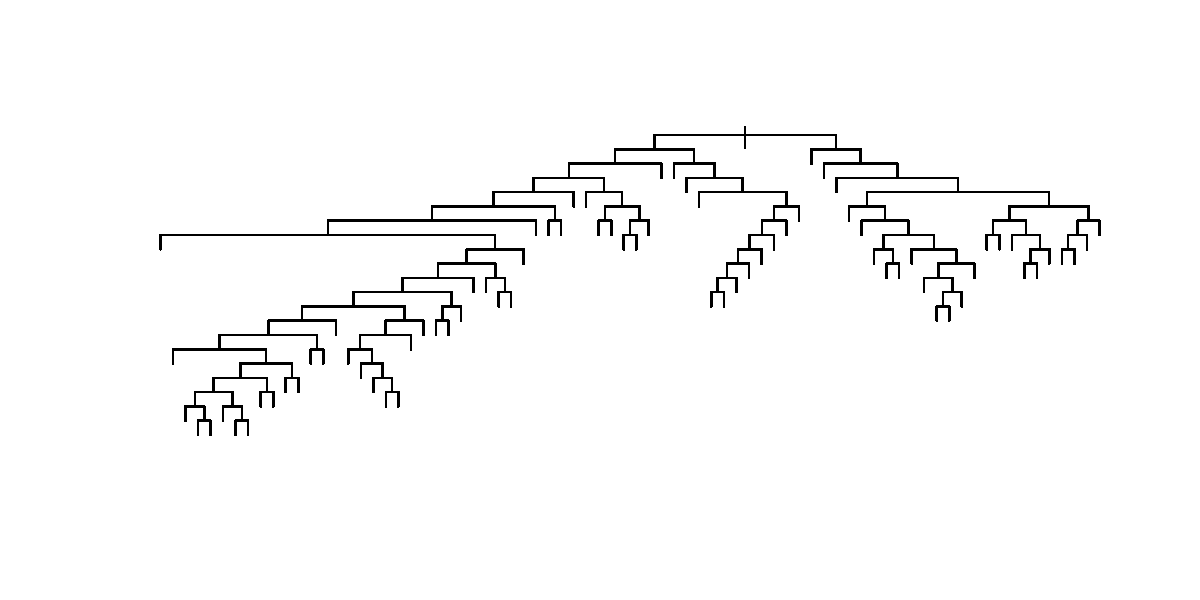
\includegraphics[angle=90]{Spam/rpartTree00001.pdf}
\caption{Classification tree for spam built using a complexity
paramater value of 0.00001 in the call to \Sfunc{rpart}}
\label{fig:rpartTree00001}
\end{figure}
\end{comment}

\begin{verbatim}
load("knnData.rda")
library(rpart)

#Convert logicals to factors
factorVars = as.data.frame(
                  lapply(derivedEmails[,logVars],as.factor))
rpartVars = cbind(factorVars, derivedEmails[,conVars])

#Fit a classification tree to classify spam
rpartFit = rpart(isSpam ~ ., data = rpartVars, 
                 method = "class")

plot(rpartFit, uniform = TRUE)
text(rpartFit)

# Fit a classification tree with smaller complexity parameter
rpartFit0001 = rpart(isSpam ~ ., data = rpartVars, 
                method="class", 
                control = rpart.control(cp=0.0001) )

# Classify the original data using the tree
oPreds0001 = predict(rpartFit0001, 
                newdata = rpartVars[,names(rpartVars) != "isSpam"], 
		type="class")

# Compute the type I and II errors 
> 1 - sum(as.logical(oPreds0001) & derivedEmails[,1])
          /sum(derivedEmails[,1]) 
[1] 0.09830508
> sum(as.logical(oPreds0001) & (!derivedEmails[,1]))
         /sum(1-derivedEmails[,1]) 
[1] 0.02076044

# Try classification on the new email messages, using the 
# tree obtained from derivedEmails
newFactorVars = as.data.frame(lapply(newEmails[,logVars],
                                     as.factor))
newRpartVars = cbind(newFactorVars, newEmails[,contVars])

nPreds00001 = predict(rpartFit0001, 
               newdata =
                 newRpartVars[,names(newRpartVars) != "isSpam"], 
                              type="class")

# The Type I and II errors shoot up 
> 1 - sum(as.logical(nPreds0001) & newEmails[,1])
          /sum(newEmails[,1]) 
[1] 0.18
> sum(as.logical(nPreds0001) & (!newEmails[,1]))
          /sum(1-newEmails[,1])
[1] 0.086
\end{verbatim}

A small complexity parameter produces a tree with more branches
%(Figure~\ref{fig:rpartTree00001}), 
and we can reduce the Type I and
II errors to 2\% and 10\% respectively. 
Table  shows the Type I and II errors for various values
of the complexity parameter.
Both errors reduce as the complexity parameter shrinks,
but when applied to the new email messages both
types of errors are much larger.
In comparison to $k^{th}$ nearest neighbor,
the best fitted tree when applied to
the new email messages does no better 
in terms of Type II error, but is 
a big improvement for Type I error.

\begin{table}
\begin{tabular}{rrrrr}
       &  \multicolumn{2}{c}{Old Mail} & \multicolumn{2}{c}{New Mail} \\
Complexity Parameter       & Type I & Type II & Type I  & Type II  \\
0.01 & 0.151 & 0.177 & 0.196 & 0.340 \\
0.005 & 0.037 & 0.190  & 0.154  & 0.208 \\
0.001 & 0.027 & 0.086  & 0.102 & 0.132 \\
0.0001 & 0.021 & 0.098 & 0.086  & 0.18 \\
0.00001 & 0.021 & 0.098 & 0.086  & 0.18 \\
\end{tabular}
\end{table}
